\documentclass[11pt,a4paper]{article}
\usepackage{kotex}
\IfFontExistsTF{UnBatang.ttf}{
 \setmainhangulfont{UnBatang.ttf}[BoldFont=UnBatangBold.ttf,
 ItalicFont=UnBatang.ttf,BoldItalicFont=UnBatangBold.ttf,Script=Hangul,Language=Korean]
}{}
\usepackage[margin=23mm,headheight=16pt]{geometry}
\usepackage{amsmath,amssymb,mathtools,bm,booktabs,tabularx,array,longtable}
\usepackage[dvipsnames]{xcolor}
\usepackage{tikz,pgfplots}
\usetikzlibrary{arrows.meta,positioning,calc}
\usepgfplotslibrary{groupplots}
\pgfplotsset{compat=1.18}
\usepackage{enumitem,fancyhdr,xurl,float,needspace,listings}
\usepackage[unicode,colorlinks=true,linkcolor=MidnightBlue,citecolor=MidnightBlue,
 urlcolor=MidnightBlue,pdftitle={PADS PD/ET MantisV2 미세 조정 기술 보고서}]{hyperref}
\definecolor{navy}{HTML}{224C70}
\definecolor{orangeplot}{HTML}{D27A27}
\definecolor{greenplot}{HTML}{3F8064}
\definecolor{redplot}{HTML}{B44446}
\definecolor{purpleplot}{HTML}{8560A6}
\definecolor{softgray}{HTML}{F4F6F8}
\newcommand{\R}{\mathbb{R}}
\newcommand{\ind}{\mathbf{1}}
\newcommand{\code}[1]{\texttt{\detokenize{#1}}}
\DeclareMathOperator{\BA}{BA}
\DeclareMathOperator{\concat}{concat}
\setlength{\parindent}{0pt}\setlength{\parskip}{.4em}
\setlength{\emergencystretch}{2.5em}
\renewcommand{\arraystretch}{1.16}
\clubpenalty=10000\widowpenalty=10000
\setlist[itemize]{leftmargin=1.5em,itemsep=.2em,topsep=.3em}
\setlist[enumerate]{leftmargin=1.8em,itemsep=.25em,topsep=.3em}
\renewcommand{\abstractname}{초록}\renewcommand{\contentsname}{목차}
\renewcommand{\figurename}{그림}\renewcommand{\tablename}{표}\renewcommand{\refname}{참고문헌}
\setcounter{tocdepth}{1}\numberwithin{equation}{section}
\pagestyle{fancy}\fancyhf{}
\fancyhead[L]{\small\color{navy}PADS PD/ET: MantisV2 미세 조정}
\fancyhead[R]{\small 기술 보고서}\fancyfoot[C]{\thepage}
\renewcommand{\headrulewidth}{.3pt}
\lstset{basicstyle=\ttfamily\footnotesize,backgroundcolor=\color{softgray},
 frame=single,rulecolor=\color{gray!25},breaklines=true,columns=fullflexible,
 keepspaces=true,showstringspaces=false}
\newenvironment{keybox}{\begin{center}\begin{minipage}{.94\linewidth}\color{navy}\hrule\vspace{.6em}\small}
 {\vspace{.5em}\hrule\end{minipage}\end{center}}
\title{\color{navy}\bfseries PADS PD/ET 분류를 위한\\[.3em]
 MantisV2 미세 조정 기술 보고서\\[.6em]
 \large Head-only/Last-block 비교, 클래스 불균형과 PR-AUC 분석}
\author{PD/ET Classification Project}
\date{2026년 11월 9일 개정\\[.25em]\small Head-only: \code{20261109T032315873662Z}\\
 Last-block: \code{20261109T041659480074Z}}

\begin{document}
\maketitle\thispagestyle{empty}
\begin{abstract}
PADS v1.0.0의 파킨슨병(PD) 276명과 본태성 떨림(ET) 28명을 대상으로
사전학습 MantisV2의 인코더를 고정한 head-only와 세 번째 Transformer 블록을
학습하는 last-block을 비교하였다.
11개 과제 구간, 양측 손목의 가속도계 및 자이로스코프에서 구성한 132채널을 사용하고,
참가자 단위 외부 5-fold, 내부 3-fold, 1회 반복으로 평가하였다.
고정 MantisV2+ridge 및 MultiROCKET--HYDRA도 같은 입력과 중첩 분할로 비교하였다.
Head-only의 pooled 균형 정확도(BA)는 81.57\%, ET 민감도는 92.86\%(26/28),
PD 특이도는 70.29\%(194/276)였다. Last-block은 각각
76.76\%, 57.14\%(16/28), 96.38\%(266/276)였다.
ET 양성 PR-AUC는 사다리꼴 적분으로 head-only 0.6391, last-block 0.6463이었고,
MCC는 각각 0.3815, 0.5534였다.
따라서 \textbf{last-block은 head-only보다 BA가 높지 않았으며,
PD 오분류를 줄이는 대신 ET 검출을 낮춘 상충 관계}를 보였다.
두 모드의 BA, PR-AUC/AP, G-mean, MCC, macro-F1을 함께 해석한다.
새 last-block 재실행의 외부 예측과 저장 텐서는 이전 실행과 정확히 같았으나,
동일 seed/참가자/분할의 반복이므로 독립 표본 증가로 계산하지 않는다.
모든 결과는 저장 자료에서 다시 계산하였다. 재학습이나 모델 순전파는 수행하지 않았으며,
단일 코호트의 탐색적 비교로 외부 임상 타당성이나 전반적 우월성을 확립하지 않는다.
\end{abstract}
\begin{keybox}
\textbf{핵심 기준.} 양성은 ET($y=1$), 음성은 PD($y=0$)다.
독립 분석 단위는 참가자이며, 모든 과제와 양측 손목 신호가 같은 fold에 속한다.
ET 비율은 9.21\%로, 모두 PD로 예측해도 일반 정확도는 90.79\%이다.
분류 임계값은 평가 전에 고정한 점수 0이며, 출력은 보정된 확률이 아니다.
전체 304명으로 적합한 최종 모델과 내부 선택 점수는 외부 평가 성능과 구분한다.
\end{keybox}
\clearpage
\tableofcontents
\vfill
\begin{keybox}
\textbf{자료와 범위.} 본문은 새 132채널 \code{head-only}/\code{last-block} 실행을 비교하고
이전 last-block 실행의 재현 여부를 확인한다.
이전 60채널 시간 표현/과제 상호작용 실험과 입력 범위가 다르다.
새로 계산한 PR-AUC와 G-mean은 보고서의 추가 분석이며,
기존 실행의 내부 후보 선택이나 임계값을 변경하지 않는다.
\end{keybox}
\clearpage

\section{연구 질문과 완료 실행}
본 실험은 외부 사전학습 시계열 표현을 PADS의 PD/ET 감별 문제에 적응시키면
고정 특징 기반 분류보다 성능이 높아지는지를 평가한다.
MantisV2는 합성 시계열 사전학습과 중간층 표현을 사용하는 기반 모델이다\cite{mantis}.
동일한 세 번째 층 표현을 출발점으로 head-only는 새로운 이진 head만,
last-block은 head와 마지막 활성 Transformer 블록을 함께 학습한다.

\begin{table}[H]\centering\small
\caption{공통 실행 규약. 개별 실행 시간은 표~\ref{tab:runs}에 제시한다.}\label{tab:run}
\begin{tabularx}{\linewidth}{@{}lX@{}}\toprule
항목 & 저장된 값\\\midrule
실행 상태 & \code{complete}\\
입력 / 모드 & \code{all}, $(304,132,976)$ / \code{head-only}, \code{last-block}\\
평가 & 외부 5-fold, 내부 3-fold, 1회 반복, seed 20261017\\
계산 환경 & macOS 26.6 arm64, Apple MPS, CPU 스레드 4개\\
저장 옵션 & \code{--fit-final}, \code{--save-outer-models} 모두 사용\\
추가 비교군 & 동일 132채널 Frozen MantisV2+ridge, MultiROCKET--HYDRA\\\bottomrule
\end{tabularx}
\end{table}

기존 고정 MantisV2 결과를 확인한 뒤 설계한 후속 연구이므로,
중첩 교차검증을 사용하더라도 결과는 탐색적으로 해석한다.
고정 MantisV2+ridge와 신경망 head의 비교는 분류기와 목적함수도 바뀐다.
기존 고정 모델은 클래스 가중 ridge 분류기이고,
두 신경망 모드는 같은 dropout 선형 head와 가중 이진 교차엔트로피를 사용한다.
이번에 완료된 \code{head-only} 대조군으로 인코더 적응의 추가 효용을 비교한다.
각 모드의 epoch는 내부 검증에서 별도로 선택하므로 비교 대상은
\textbf{조정된 두 학습 절차}이며 epoch를 고정한 적응의 단일 효과와 구분한다.

원래 연구 목표는 과제 내 떨림의 시간적 역학과 과제 간 상호작용을 명시적으로 결합하는 것이다.
이번 모델에는 채널 간 attention이나 과제 간 곱항 모듈이 없다.
각 채널의 비선형 표현을 연결하고 선형 head로 합산하므로,
이번 결과는 \textbf{인코더 적응 여부의 비교}이며 원래 과제 상호작용 모듈의 효과 검증은 아니다.
\clearpage

\section{데이터와 클래스 불균형}
\subsection{참가자와 정답}
자료는 PADS v1.0.0\cite{pads,padsstudy}의 공식 전처리 movement 이진 파일이다.
참가자 $i\in\{1,\ldots,N\}$에 대해 $N=304$이며,
진단 문자열이 \code{Parkinson's}이면 $y_i=0$,
\code{Essential Tremor}이면 $y_i=1$로 정한다.
PD 276명, ET 28명으로,
\begin{equation}
 \pi_{\mathrm{ET}}=\frac{28}{304}=0.092105\ldots,\qquad
 \frac{N_{\mathrm{PD}}}{N_{\mathrm{ET}}}=\frac{276}{28}=9.8571\ldots.
\end{equation}
원래 숫자 라벨 2에는 ET 외의 감별진단도 있으므로 이를 ET 라벨로 사용하지 않는다.
PD로 배정되었지만 설명에 ET가 언급된 8명은 공식 PD 라벨을 유지한다.
진단 설명, 인구학적 변수, 설문, 약물 및 참가자 ID는 모델 입력에서 제외한다.

불균형은 세 단계에서 다룬다. 첫째, 층화한 참가자 분할을 사용한다.
둘째, 각 적합의 학습 참가자만으로 역빈도 클래스 가중치를 계산한다.
셋째, 평가는 일반 정확도를 주 지표로 삼지 않고 BA와 소수 클래스 지표를 함께 사용한다.
가중 손실은 ET의 총 손실 기여도를 높이지만, ET 참가자 28명의 정보량 자체를 늘리지는 않는다.
이번 실행에는 과표집, SMOTE나 합성 ET 참가자 생성이 없다.

\subsection{132채널 입력의 정의}
참가자 신호를 $X_i\in\R^{C\times L}$, $C=132$, $L=976$으로 정의한다.
132는 동시 측정 물리 축의 수가 아니라 다음 조합의 수다.
\begin{equation}
 C=11\text{개 구간}\times2\text{개 손목}\times2\text{개 센서}\times3\text{개 축}.
\end{equation}
가속도계와 자이로스코프의 XYZ 순서를 유지하며, 구간 순서는 다음과 같다.
\begin{quote}\small
\code{Relaxed1}, \code{Relaxed2}, \code{RelaxedTask1}, \code{RelaxedTask2},
\code{StretchHold}, \code{HoldWeight}, \code{DrinkGlas}, \code{CrossArms},
\code{TouchNose}, \code{Entrainment1}, \code{Entrainment2}.
\end{quote}
인지 부하 안정 과제는 안정 자세에서의 연속 7 빼기다.
이번 실행은 안정/인지/자세의 다섯 구간만 사용하는 60채널 설정보다 범위가 넓다.
따라서 그 이전 60채널 모델의 수치와 직접 대응 비교하지 않는다.

\subsection{전처리와 시간축의 한계}
공식 전처리의 가속도 중력 보정, 과제 선택, 구간 분할과 crop을 유지한다.
긴 기록은 1024표본 구간으로 나뉘고 각 구간 앞 48표본을 제거하여 976표본을 남긴다.
명목상 표본율은 100\,Hz지만, 이진 입력은 표본 인덱스 기반이다.
원시 timestamp의 불규칙 간격이나 누락을 이번 코드가 복원하지 않는다.
추가적인 원신호별 z-score는 적용하지 않는다.
이후 $976\to512$ 선형 보간은 모델 길이 맞춤이며, timestamp 재표본화나
antialias 저역통과 필터링을 대신하지 않는다.
\clearpage

\section{MantisV2 분류 모델}
\subsection{고정된 초기 체크포인트와 활성 경로}
패키지는 \code{mantis-tsfm==1.1.0}, 모델은 \code{paris-noah/MantisV2}이며,
revision은 다음으로 고정한다.
\begin{quote}\small\code{99fe0f548960e272fbfa4b82fd9b5b5956779dfd}\end{quote}
전체 6블록 체크포인트를 먼저 엄격하게 불러와 해시와 텐서 이름/형상을 검증한 뒤,
세 번째 층 뒤의 사용하지 않는 3블록을 제거한다.
\code{return_transf_layer=2}는 0부터 세는 층 번호이므로 세 번째 블록이다.
원본 사전학습 가중치 파일은 수정하지 않는다.

\begin{table}[H]\centering\small
\caption{132채널 \code{last-block} 모델의 파라미터 수. 정규화 buffer는 제외한다.}
\begin{tabularx}{\linewidth}{@{}Xr@{}}\toprule
객체 & 파라미터 수\\\midrule
원본 6블록 사전학습 체크포인트 & 4,188,672\\
3블록으로 자른 인코더(사용하지 않는 projector 포함) & 2,214,144\\
학습하는 세 번째 Transformer 블록 & 658,176\\
새 참가자 선형 head(가중치와 bias) & 67,585\\
warmup 이후 학습 가능한 합계 & 725,761\\
저장된 모델의 전체 파라미터 & 2,281,729\\\bottomrule
\end{tabularx}
\end{table}
사용하지 않는 사전학습 projector 66,304개 파라미터는 저장되지만 고정되어 있다.
Last-block의 첫 epoch에는 head만 갱신하며, 이후 세 번째 블록도 갱신한다.
앞의 토큰 생성부와 첫 두 블록은 고정하고 평가 모드를 유지한다.
Head-only에서는 인코더 전체를 고정하여 학습 가능한 파라미터가 head의
67,585개뿐이다. 저장된 전체 파라미터 수는 두 모드가 같으며,
head-only가 학습 파라미터를 줄여도 저장/추론용 인코더 자체가 작아지는 것은 아니다.
저장 텐서를 초기 체크포인트와 비교해 head-only의 모든 인코더 텐서가
정확히 유지되고 last-block의 세 번째 블록만 실제 변경됨을 확인했다.
코드의 \code{full} 옵션도 선택된 세 번째 층까지의 활성 경로 전체를 의미한다.
원본 여섯 블록 전체를 학습한 결과는 이번 보고서에 없다.

\subsection{채널별 표현과 참가자 점수}
참가자 $i$의 채널 $c$를 $x_{ic}\in\R^{976}$이라 하자.
선형 보간 연산 $\mathcal I:\R^{976}\to\R^{512}$는
\code{align_corners=False}로 적용한다.
인코더 $f_\theta:\R^{512}\to\R^{512}$는 모든 채널에서 가중치를 공유하지만
각 채널을 독립적으로 처리한다.
세 번째 블록의 class token $h_{\mathrm{cls}}^{(3)}\in\R^{256}$과
32개 patch token $h_j^{(3)}\in\R^{256}$을 사용해
\begin{equation}
 z_{ic}(\theta)=f_\theta(\mathcal I x_{ic})
 =\concat\!\left(h_{\mathrm{cls}}^{(3)},\frac1{32}\sum_{j=1}^{32}h_j^{(3)}\right)\in\R^{512}.
\end{equation}
활성 Transformer 설정은 hidden dimension 256, head 8개, head dimension 32,
feed-forward dimension 512, dropout 0.1이다.
사전학습 토큰 생성기의 내부 신호 정규화와 원래 patch 평균/표준편차 경로를 보존한다.
\begin{equation}
 z_i(\theta)=\concat(z_{i1}(\theta),\ldots,z_{i132}(\theta))\in\R^{67584}.
\end{equation}
여기서 채널 순서는 고정되며, 서로 다른 채널을 시간축으로 이어 붙이지 않는다.

\subsection{학습 참가자만 사용하는 고정 정규화}
한 번의 적합에 사용되는 학습 참가자 집합을 $A$라 하고 초기 인코더를 $\theta_0$라 하자.
먼저 완전히 고정된 외부 사전학습 인코더로 $z_i(\theta_0)$를 계산한다.
각 특징 $d\in\{1,\ldots,67584\}$의 정규화 통계는
\begin{align}
 \mu_{A,d}&=\frac1{|A|}\sum_{i\in A}z_{i,d}(\theta_0),\\
 \sigma_{A,d}&=\left[\frac1{|A|}\sum_{i\in A}(z_{i,d}(\theta_0)-\mu_{A,d})^2\right]^{1/2},\\
 a_{A,d}&=\begin{cases}1,&\sigma_{A,d}<10^{-6},\\\sigma_{A,d},&\text{그 외}.
 \end{cases}
\end{align}
평균과 표준편차는 float64로 계산한 후 float32 buffer로 저장한다.
적응 중에도 $\mu_A,a_A$는 다시 적합하지 않는다.
현재 인코더의 표현을 초기 표현에서 얻은 같은 좌표계로 정규화한다.
학습 시 dropout을 $D_{0.1}$이라 하면 점수는
\begin{equation}\label{eq:score}
 s_i=\bm w^\top D_{0.1}\!\left((z_i(\theta)-\bm\mu_A)\oslash\bm a_A\right)+b,
 \qquad \widehat y_i=\ind\{s_i>0\}.
\end{equation}
$\oslash$는 원소별 나눗셈, $\bm w\in\R^{67584}$, $b\in\R$다.
평가 때 dropout은 항등 연산이며, 점수 0은 PD로 분류한다.

초기 고정 특징의 전체 코호트 cache는 PADS 참가자 간 통계를 적합하지 않아 공유할 수 있다.
반면 정규화는 내부/외부 적합마다 해당 학습 집합에서 다시 계산한다.
두 모드 모두 원신호에서 $z_i(\theta)$를 매번 다시 계산한다.
Head-only에서는 항상 $\theta=\theta_0$이며 인코더 gradient를 계산하지 않는다.
적응된 특징이나 학습된 인코더를 다른 fold에 재사용하지 않는다.

\begin{figure}[H]\centering
\begin{tikzpicture}[node distance=5mm,>=Latex,
 box/.style={draw=navy,rounded corners=2pt,fill=navy!4,align=center,text width=.79\linewidth,minimum height=9mm,font=\small}]
\node[box](x){참가자 원신호: $132\times976$};
\node[box,below=of x](i){채널별 선형 보간: $132\times512$};
\node[box,below=of i](e){공유 MantisV2: 토큰 생성부 + 첫 두 블록 고정\\Head-only: 세 번째도 고정 / Last-block: 세 번째 학습};
\node[box,below=of e](z){채널별 512차원 표현을 순서대로 연결: $67{,}584$차원};
\node[box,below=of z](s){학습 집합의 초기 특징 통계로 정규화\\Dropout(0.1) + 선형 head $\to$ ET logit};
\draw[->](x)--(i);\draw[->](i)--(e);\draw[->](e)--(z);\draw[->](z)--(s);
\end{tikzpicture}
\caption{한 참가자의 순전파. 채널 간 attention이나 명시적 과제 곱항은 없다.}
\end{figure}
\clearpage

\section{불균형을 고려한 학습과 계산 절차}
\subsection{클래스 가중 목적함수}
학습 집합 $A$의 클래스 수를 $n_{A,c}=|\{i\in A:y_i=c\}|$라 하면
\begin{equation}
 \omega_{A,c}=\frac{|A|}{2n_{A,c}},\qquad c\in\{0,1\}.
\end{equation}
이 값은 \textbf{각 내부/외부/최종 적합의 학습 집합에서} 다시 계산한다.
전체 코호트에서는 $\omega_{A,0}=0.550725$, $\omega_{A,1}=5.428571$이다.

$\ell(y,s)=\log(1+e^s)-ys$를 수치적으로 안정한
\code{binary_cross_entropy_with_logits}로 계산한다. 학습 목적의 데이터 항은
\begin{align}
 \mathcal L_A(\theta,\bm w,b)
 &=\frac1{|A|}\sum_{i\in A}\omega_{A,y_i}\ell(y_i,s_i)\\
 &=\frac12\left[\frac1{n_{A,0}}\sum_{i\in A:y_i=0}\ell(0,s_i)
 +\frac1{n_{A,1}}\sum_{i\in A:y_i=1}\ell(1,s_i)\right].\label{eq:weighted}
\end{align}
두 클래스 평균 손실의 기여도는 각각 $1/2$다. 배치는 원래 비율에서 무작위로 섞으므로
개별 microbatch의 클래스 수는 불균형할 수 있다.
$\operatorname{sigmoid}(s_i)$를 원래 유병률에 보정된 확률로 해석하지 않는다.

\subsection{최적화와 gradient accumulation}
AdamW\cite{adamw}의 head LR은 $10^{-4}$, last-block의 인코더 LR 후보는
$\{10^{-5},3\times10^{-5}\}$, decay는 $0.01$이다. Head-only의 인코더 LR 0은
고정을 나타내며, encoder parameter group은 optimizer에 포함하지 않는다.
모멘트와 분리된 weight decay는 $\mathcal L_A+\lambda\|\theta\|_2^2$의 Adam 최적화와 다르다.
$\beta_1=0.9$, $\beta_2=0.999$, $\epsilon=10^{-8}$이며 scheduler/혼합 정밀도는 없다.

참가자 2명의 microbatch 8개를 누적하여 보통 16명당 한 번 갱신한다.
불완전한 마지막 group도 포함하여 group $G$의 microbatch $B\subseteq G$ 손실은
\begin{equation}
 \mathcal L_B=\frac1{|G|}\sum_{i\in B}\omega_{A,y_i}\ell(y_i,s_i).
\end{equation}
분모는 실제 참가자 수 $|G|$다. group의 gradient를 누적하고 norm을 최대 1로 자른 뒤 갱신한다.
Last-block의 첫 epoch는 총 epoch에 포함되는 head-only warmup이다.
3 epoch를 선택하면 head-only 1회와 공동 학습 2회다.
Head-only 모드는 모든 epoch에서 head만 학습하므로 별도 warmup 전환이 없고,
이력의 \code{head_warmup}은 전부 \code{False}다.

한 번에 16개 채널 기록을 처리하고 비재진입 activation checkpointing으로 역전파 시 활성값을
재계산한다. 이는 메모리를 줄이고 계산량을 늘린다. chunking만으로 전체 그래프 저장을 피할 수는 없다.
검증은 \code{no_grad}/평가 모드다. 고정 모듈은 평가 모드, 적응하는 세 번째 블록만 학습 모드다.

\subsection{seed와 적합 횟수}
분할 seed는 20261017이며 모델 seed는 결정적으로 파생한다(부록~\ref{app:splits}).
seed는 초기 head, 섞기, 확률적 연산을 통제한다. 장치 간 bit 단위 재현성을 보장하지 않는다.

LR 후보 수를 $m$이라 하면 각 외부 fold에 내부 $3m$개 trajectory와 재적합 1개가 필요하다.
전체 코호트의 별도 선택/최종 적합까지 포함한 횟수는
\begin{equation}
 5(3m+1)+(3m+1)=\begin{cases}
 42\;(35+7),&m=2\quad\text{(Last-block)},\\
 24\;(20+4),&m=1\quad\text{(Head-only)}.
 \end{cases}
\end{equation}
\clearpage

\section{참가자 단위 중첩 교차검증}
\subsection{내부 선택과 외부 평가}
전체 참가자 집합을 $I$, 외부 fold $k$의 평가 집합을 $T_k$,
학습 집합을 $A_k=I\setminus T_k$라 하자. $T_1,\ldots,T_5$는 서로소이며
합집합은 $I$다. 모든 과제, 양측 손목과 내부 patch가 같은 참가자와 함께 이동한다.
외부 평가자는 fold마다 ET 5--6명, PD 55--56명이다.

내부 후보는 $\eta_e\in\{10^{-5},3\times10^{-5}\}$,
$\lambda=0.01$, $E\in\{3,5,10\}$의 6개 조합(last-block)이다.
Head-only는 $\eta_e=0$과 같은 epoch 집합의 3개 조합을 평가한다.
내부 검증 집합 $V_{k,j}$, $j=1,2,3$에 대한 BA의 산술평균
\begin{equation}
 Q_k(\eta_e,\lambda,E)=\frac13\sum_{j=1}^3
 \BA\bigl(\{y_i,\widehat y_i^{(k,j;\eta_e,\lambda,E)}:i\in V_{k,j}\}\bigr)
\end{equation}
을 최대화한다. $10^{-12}$ 이내 동률이면 더 큰 decay, 더 적은 epoch,
더 작은 인코더 학습률 순으로 선택한다.
이후 초기 체크포인트와 새 head에서 출발하여 $A_k$ 전체로 선택 epoch만큼 다시 학습하고
$T_k$를 한 번 예측한다. 외부 점수로 early stopping이나 임계값 선택을 하지 않는다.

\begin{table}[H]\centering\small
\caption{내부 검증으로 선택된 설정. SD는 3개 내부 fold BA의 기술적 표준편차다.}
\begin{tabular}{@{}llrrrr@{}}\toprule
모드 & Fold & 인코더 LR & 총 epoch & 내부 평균 BA(\%) & SD(pp)\\\midrule
Head-only & 1 & 0e+00 & 3 & 81.52 & 7.98 \\
Head-only & 2 & 0e+00 & 10 & 85.50 & 5.95 \\
Head-only & 3 & 0e+00 & 10 & 81.99 & 6.48 \\
Head-only & 4 & 0e+00 & 10 & 82.91 & 2.57 \\
Head-only & 5 & 0e+00 & 3 & 83.65 & 6.12 \\
Head-only & Final & 0e+00 & 5 & 79.19 & 4.29 \\
Last-block & 1 & 1e-05 & 3 & 76.35 & 16.98 \\
Last-block & 2 & 1e-05 & 3 & 79.35 & 3.18 \\
Last-block & 3 & 1e-05 & 3 & 74.64 & 8.35 \\
Last-block & 4 & 1e-05 & 3 & 69.31 & 14.58 \\
Last-block & 5 & 3e-05 & 10 & 81.31 & 4.95 \\
Last-block & Final & 1e-05 & 3 & 79.68 & 3.58 \\
\bottomrule\end{tabular}
\end{table}
각 Final 행은 외부 평가가 끝난 뒤 전체 코호트에서 별도로 시행한 선택이다.
모든 행의 head 학습률은 $10^{-4}$, weight decay는 $0.01$이다.
Last-block의 외부 1--4번 fold와 최종 적합은 3 epoch를,
5번 fold는 가장 큰 LR과 10 epoch를 선택했다.
Head-only는 외부 1/5번 fold에서 3 epoch, 2/3/4번에서 10 epoch,
최종 적합에서 5 epoch를 선택했다.
일부 선택이 탐색 경계에 있으므로 전역적인 최적 설정을 찾았다고 주장하지 않는다.

\subsection{비교군과 대응성}
Frozen MantisV2는 같은 체크포인트, 층, token 결합, 보간과 132채널 입력을 사용한다.
고정 특징에 학습 집합만의 StandardScaler를 적합하고,
클래스 가중 ridge의 $\alpha$를 다음 집합에서 같은 내부 평균 BA로 선택한다.
\begin{equation*}
 \alpha\in\{10^{-3},10^{-2},10^{-1},1,10,100,1000\}.
\end{equation*}
다섯 fold 모두 $\alpha=1000$을 선택했다.
MultiROCKET--HYDRA\cite{multirocket,hydra}도 같은 코호트, 입력과 중첩 분할에서
특징 변환/스케일러를 각 학습 집합에 적합한 뒤 가중 ridge로 분류한다.
저장된 설정은 MultiROCKET kernel 요청 6250개, HYDRA 64그룹, 그룹당 8개 kernel이다.
네 방법의 데이터 파일 해시, 참가자 순서와 외부/내부 분할이 모두 일치함을 확인하였다.
\clearpage

\section{불균형을 반영한 평가 지표}
\subsection{혼동행렬과 고정 임계값 지표}
양성 ET를 기준으로 $TP$는 ET를 ET로, $FN$은 ET를 PD로,
$TN$은 PD를 PD로, $FP$는 PD를 ET로 분류한 참가자 수다.
혼동행렬은 실제 행/예측 열 순서가 PD, ET인
\begin{equation}
 \begin{pmatrix}TN&FP\\FN&TP\end{pmatrix}
\end{equation}
으로 제시한다. $R_{\mathrm{ET}}=TP/(TP+FN)$는 ET 민감도이고,
$R_{\mathrm{PD}}=TN/(TN+FP)$는 PD 특이도다.
\begin{align}
 \BA&=\tfrac12(R_{\mathrm{ET}}+R_{\mathrm{PD}}), &
 G\text{-mean}&=\sqrt{R_{\mathrm{ET}}R_{\mathrm{PD}}},\\
 P_{\mathrm{ET}}&=\frac{TP}{TP+FP}, &
 \mathrm{Accuracy}&=\frac{TP+TN}{N}.
\end{align}
BA는 각 클래스 재현율에 같은 비중을 준다.
G-mean은 한 클래스 재현율이 0이면 0이어서 한쪽만 분류하는 모델을 드러낸다.
일반 정확도는 이 코호트에서 PD가 많아 쉽게 높아진다.
모두 PD인 분류기는 정확도 90.79\%, BA 50\%, G-mean 0이다.

\begin{align}
 F_{1,\mathrm{ET}}&=\frac{2TP}{2TP+FP+FN},\qquad
 F_{1,\mathrm{PD}}=\frac{2TN}{2TN+FP+FN},\\
 \mathrm{Macro}\text{-}F_1&=\tfrac12(F_{1,\mathrm{ET}}+F_{1,\mathrm{PD}}),\\
 \mathrm{MCC}&=\frac{TP\,TN-FP\,FN}
 {\sqrt{(TP+FP)(TP+FN)(TN+FP)(TN+FN)}}.
\end{align}
MCC는 혼동행렬의 네 칸을 사용하고 $[-1,1]$ 범위의 상관 형태 지표다\cite{mcc}.
Macro-F1은 클래스별 F1을 동일 비중으로 평균한다.
둘 다 불균형에서 보완적인 정보를 제공하지만 유병률과 무관한 지표는 아니다.
F1/MCC의 분모가 0인 퇴화 경우에는 scikit-learn의 0 처리 규약을 따른다.
가중 평균 F1은 다수 클래스가 다시 우세해질 수 있어 주 지표로 쓰지 않는다.

\newpage
\subsection{PR-AUC와 Average Precision을 명시적으로 구분}
임계값 $t$에서 $\widehat y_i(t)=\ind\{s_i>t\}$라 하고
recall $R(t)$와 precision $P(t)$를 정의한다.
모든 서로 다른 점수와 표준 끝점을 사용한 PR 좌표를 recall 증가 순서로
$(R_j,P_j)$, $j=0,\ldots,m$이라 하면 본 보고서의 \textbf{PR-AUC}는
\begin{equation}\label{eq:prauc}
 \mathrm{PR}\text{-}\mathrm{AUC}_{\mathrm{trap}}
 =\sum_{j=1}^{m}(R_j-R_{j-1})\frac{P_j+P_{j-1}}2.
\end{equation}
구현은 \code{precision_recall_curve(y, score)}와 \code{auc(recall, precision)}다.
정답 이진 예측값이 아닌 \textbf{연속 점수}를 사용하며 ET가 양성이다.
그림의 PR 좌표는 직선으로 연결하므로 식~\eqref{eq:prauc}의 적분 규칙과 대응한다.

반면 AP는 recall 증분에 해당 precision을 가중한 계단형 요약이다\cite{sklearnap}.
정확히는 라이브러리가 반환하는 recall 감소 순서 $r_0\ge\cdots\ge r_m$와
precision $p_j$에 대해
\begin{equation}
 \mathrm{AP}=\sum_{j=0}^{m-1}(r_j-r_{j+1})p_j.
\end{equation}
따라서 \textbf{AP를 사다리꼴 PR-AUC와 동일한 수치로 표기하지 않는다.}
두 적분값 모두 직접 합 공식으로 다시 계산하여 라이브러리 결과와 일치함을 확인했다.
두 지표는 특정 임계값 하나에 의존하지 않지만 양성 비율과 표본 구성에는 의존한다.

무정보 순위의 PR 참조선은 $P=\pi_{\mathrm{ET}}=0.0921$이다.
이는 이론적인 수평 참조선이며 유한 표본의 모든 난수 점수 적분이 정확히 이 값이라는 뜻은 아니다.
상수 점수만 갖는 Always PD 모델은 AP가 $\pi_{\mathrm{ET}}$이지만,
라이브러리의 $(R,P)=(0,1)$ 끝점과 $(1,\pi_{\mathrm{ET}})$를 직선으로 연결하면
퇴화한 사다리꼴 면적 $(1+\pi_{\mathrm{ET}})/2=0.5461$이 나온다.
이는 분별력의 근거가 아닌 \textbf{끝점 보간의 인공적 효과}다.
따라서 주 표의 Always PD PR-AUC는 대시로 표시하고 AP 0.0921을 기준으로 사용한다.
원시 계산값은 감사 JSON/CSV에 그대로 남긴다.

AUROC는 무작위 ET의 점수가 PD보다 높을 확률(동률 절반)을 요약한다.
불균형을 반영한 precision은 직접 나타내지 않아 PR-AUC 및 ET 정밀도와 같이 본다.
순위 지표를 계산하려고 임계값을 변화시키는 것은 고정 임계값 평가를 대체하거나
외부 자료에서 새 운영 임계값을 선택한다는 뜻이 아니다.
\clearpage

\section{외부 평가 결과}
\subsection{주 결과와 불균형 보완 지표}
각 참가자가 자신을 학습에 사용하지 않은 외부 모델에서 얻은 예측 한 개를 사용한다.
아래 pooled 결과는 304명의 예측을 합친 값이며 5개 fold 수치의 단순평균과 구분한다.
\begin{table}[H]\centering\small
\caption{동일 입력/분할의 외부 예측 비교. BA, ET 민감도, PD 특이도는 \% 단위다.}
\label{tab:main}\setlength{\tabcolsep}{4pt}
\begin{tabular}{@{}lrrrrr@{}}\toprule
방법 & BA & ET 민감도 & PD 특이도 & AUROC & PR-AUC\\\midrule
Head-only & 81.57 & 92.86 & 70.29 & 0.9036 & 0.6391 \\
Last-block & 76.76 & 57.14 & 96.38 & 0.8586 & 0.6463 \\
Frozen MantisV2 & 70.89 & 42.86 & 98.91 & 0.8876 & 0.6229 \\
MR--HYDRA & 67.13 & 35.71 & 98.55 & 0.9000 & 0.5557 \\
Always PD & 50.00 & 0.00 & 100.00 & 0.5000 & -- \\
\bottomrule\end{tabular}
\end{table}
\begin{table}[H]\centering\small
\caption{불균형을 고려한 보완 지표. AP는 PR-AUC와 다른 요약이며 정밀도만 \% 단위다.}
\label{tab:imbalance}\setlength{\tabcolsep}{4pt}
\begin{tabular}{@{}lrrrrrr@{}}\toprule
방법 & G-mean & MCC & Macro-F1 & ET-F1 & AP & ET 정밀도\\\midrule
Head-only & 0.8079 & 0.3815 & 0.6022 & 0.3824 & 0.6444 & 24.07 \\
Last-block & 0.7421 & 0.5534 & 0.7764 & 0.5926 & 0.6505 & 61.54 \\
Frozen MantisV2 & 0.6511 & 0.5577 & 0.7623 & 0.5581 & 0.6272 & 80.00 \\
MR--HYDRA & 0.5933 & 0.4727 & 0.7187 & 0.4762 & 0.5776 & 71.43 \\
Always PD & 0.0000 & 0.0000 & 0.4759 & 0.0000 & 0.0921 & 0.00 \\
\bottomrule\end{tabular}
\end{table}

Head-only는 BA와 G-mean이 가장 높지만 MCC와 macro-F1은 last-block보다 낮다.
두 모드의 ET 정밀도는 각각 24.07\%, 61.54\%다.
일반 정확도는 head-only 72.37\%, last-block 92.76\%,
고정 MantisV2 93.75\%, MR--HYDRA 92.76\%다.
\textbf{지표별 순위가 다르므로 단일 수치로 전반적 우위를 선언하지 않는다.}

실제 행/예측 열 순서가 PD, ET인 혼동행렬은
\begin{equation}
 \begin{gathered}
 \underbrace{\begin{pmatrix}194&82\\2&26\end{pmatrix}}_{\text{Head-only}},\qquad
 \underbrace{\begin{pmatrix}266&10\\12&16\end{pmatrix}}_{\text{Last-block}},\\[.8em]
 \underbrace{\begin{pmatrix}273&3\\16&12\end{pmatrix}}_{\text{Frozen MantisV2}},\qquad
 \underbrace{\begin{pmatrix}272&4\\18&10\end{pmatrix}}_{\text{MR--HYDRA}}.
 \end{gathered}
\end{equation}
Head-only는 ET라고 분류한 108명 중 26명, last-block은 26명 중 16명이 실제 ET다.
BA는 두 클래스 재현율을 동일하게 가중하지만 양성 예측의 정밀도를 직접 평가하지 않는다.
\clearpage

\subsection{PR 곡선과 ROC 곡선}
\begin{figure}[H]\centering
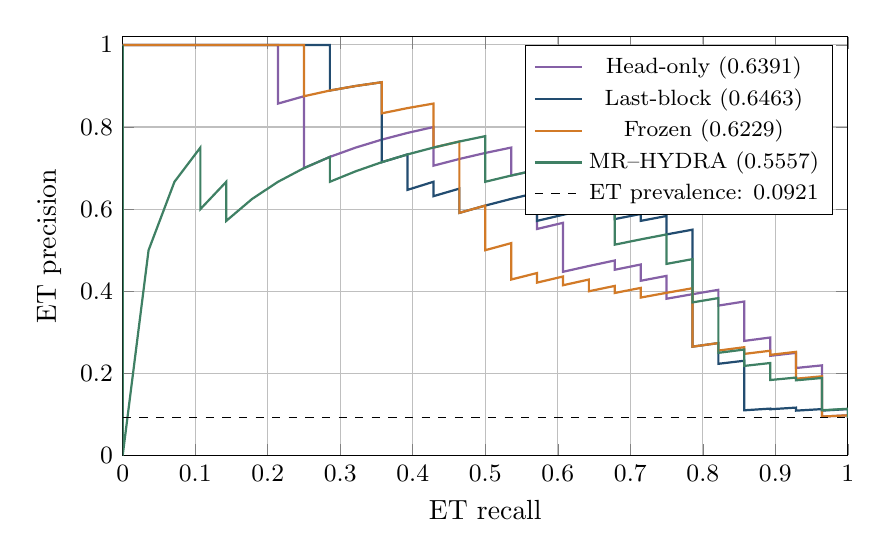
\begin{tikzpicture}
\begin{axis}[width=.89\linewidth,height=6.9cm,xmin=0,xmax=1,ymin=0,ymax=1.02,
 xlabel={ET recall},ylabel={ET precision},grid=major,
 legend style={at={(.98,.98)},anchor=north east,font=\footnotesize,fill=white},
 tick label style={font=\small}]
\addplot[purpleplot,thick] coordinates {(0.0000000,1.0000000) (0.0357143,1.0000000) (0.0714286,1.0000000) (0.1071429,1.0000000) (0.1428571,1.0000000) (0.1785714,1.0000000) (0.2142857,1.0000000) (0.2142857,0.8571429) (0.2500000,0.8750000) (0.2500000,0.7777778) (0.2500000,0.7000000) (0.2857143,0.7272727) (0.3214286,0.7500000) (0.3571429,0.7692308) (0.3928571,0.7857143) (0.4285714,0.8000000) (0.4285714,0.7500000) (0.4285714,0.7058824) (0.4642857,0.7222222) (0.5000000,0.7368421) (0.5357143,0.7500000) (0.5357143,0.7142857) (0.5357143,0.6818182) (0.5714286,0.6956522) (0.5714286,0.6666667) (0.5714286,0.6400000) (0.5714286,0.6153846) (0.5714286,0.5925926) (0.5714286,0.5714286) (0.5714286,0.5517241) (0.6071429,0.5666667) (0.6071429,0.5483871) (0.6071429,0.5312500) (0.6071429,0.5151515) (0.6071429,0.5000000) (0.6071429,0.4857143) (0.6071429,0.4722222) (0.6071429,0.4594595) (0.6071429,0.4473684) (0.6428571,0.4615385) (0.6785714,0.4750000) (0.6785714,0.4634146) (0.6785714,0.4523810) (0.7142857,0.4651163) (0.7142857,0.4545455) (0.7142857,0.4444444) (0.7142857,0.4347826) (0.7142857,0.4255319) (0.7500000,0.4375000) (0.7500000,0.4285714) (0.7500000,0.4200000) (0.7500000,0.4117647) (0.7500000,0.4038462) (0.7500000,0.3962264) (0.7500000,0.3888889) (0.7500000,0.3818182) (0.7857143,0.3928571) (0.8214286,0.4035088) (0.8214286,0.3965517) (0.8214286,0.3898305) (0.8214286,0.3833333) (0.8214286,0.3770492) (0.8214286,0.3709677) (0.8214286,0.3650794) (0.8571429,0.3750000) (0.8571429,0.3692308) (0.8571429,0.3636364) (0.8571429,0.3582090) (0.8571429,0.3529412) (0.8571429,0.3478261) (0.8571429,0.3428571) (0.8571429,0.3380282) (0.8571429,0.3333333) (0.8571429,0.3287671) (0.8571429,0.3243243) (0.8571429,0.3200000) (0.8571429,0.3157895) (0.8571429,0.3116883) (0.8571429,0.3076923) (0.8571429,0.3037975) (0.8571429,0.3000000) (0.8571429,0.2962963) (0.8571429,0.2926829) (0.8571429,0.2891566) (0.8571429,0.2857143) (0.8571429,0.2823529) (0.8571429,0.2790698) (0.8928571,0.2873563) (0.8928571,0.2840909) (0.8928571,0.2808989) (0.8928571,0.2777778) (0.8928571,0.2747253) (0.8928571,0.2717391) (0.8928571,0.2688172) (0.8928571,0.2659574) (0.8928571,0.2631579) (0.8928571,0.2604167) (0.8928571,0.2577320) (0.8928571,0.2551020) (0.8928571,0.2525253) (0.8928571,0.2500000) (0.8928571,0.2475248) (0.8928571,0.2450980) (0.8928571,0.2427184) (0.9285714,0.2500000) (0.9285714,0.2476190) (0.9285714,0.2452830) (0.9285714,0.2429907) (0.9285714,0.2407407) (0.9285714,0.2385321) (0.9285714,0.2363636) (0.9285714,0.2342342) (0.9285714,0.2321429) (0.9285714,0.2300885) (0.9285714,0.2280702) (0.9285714,0.2260870) (0.9285714,0.2241379) (0.9285714,0.2222222) (0.9285714,0.2203390) (0.9285714,0.2184874) (0.9285714,0.2166667) (0.9285714,0.2148760) (0.9285714,0.2131148) (0.9642857,0.2195122) (0.9642857,0.2177419) (0.9642857,0.2160000) (0.9642857,0.2142857) (0.9642857,0.2125984) (0.9642857,0.2109375) (0.9642857,0.2093023) (0.9642857,0.2076923) (0.9642857,0.2061069) (0.9642857,0.2045455) (0.9642857,0.2030075) (0.9642857,0.2014925) (0.9642857,0.2000000) (0.9642857,0.1985294) (0.9642857,0.1970803) (0.9642857,0.1956522) (0.9642857,0.1942446) (0.9642857,0.1928571) (0.9642857,0.1914894) (0.9642857,0.1901408) (0.9642857,0.1888112) (0.9642857,0.1875000) (0.9642857,0.1862069) (0.9642857,0.1849315) (0.9642857,0.1836735) (0.9642857,0.1824324) (0.9642857,0.1812081) (0.9642857,0.1800000) (0.9642857,0.1788079) (0.9642857,0.1776316) (0.9642857,0.1764706) (0.9642857,0.1753247) (0.9642857,0.1741935) (0.9642857,0.1730769) (0.9642857,0.1719745) (0.9642857,0.1708861) (0.9642857,0.1698113) (0.9642857,0.1687500) (0.9642857,0.1677019) (0.9642857,0.1666667) (0.9642857,0.1656442) (0.9642857,0.1646341) (0.9642857,0.1636364) (0.9642857,0.1626506) (0.9642857,0.1616766) (0.9642857,0.1607143) (0.9642857,0.1597633) (0.9642857,0.1588235) (0.9642857,0.1578947) (0.9642857,0.1569767) (0.9642857,0.1560694) (0.9642857,0.1551724) (0.9642857,0.1542857) (0.9642857,0.1534091) (0.9642857,0.1525424) (0.9642857,0.1516854) (0.9642857,0.1508380) (0.9642857,0.1500000) (0.9642857,0.1491713) (0.9642857,0.1483516) (0.9642857,0.1475410) (0.9642857,0.1467391) (0.9642857,0.1459459) (0.9642857,0.1451613) (0.9642857,0.1443850) (0.9642857,0.1436170) (0.9642857,0.1428571) (0.9642857,0.1421053) (0.9642857,0.1413613) (0.9642857,0.1406250) (0.9642857,0.1398964) (0.9642857,0.1391753) (0.9642857,0.1384615) (0.9642857,0.1377551) (0.9642857,0.1370558) (0.9642857,0.1363636) (0.9642857,0.1356784) (0.9642857,0.1350000) (0.9642857,0.1343284) (0.9642857,0.1336634) (0.9642857,0.1330049) (0.9642857,0.1323529) (0.9642857,0.1317073) (0.9642857,0.1310680) (0.9642857,0.1304348) (0.9642857,0.1298077) (0.9642857,0.1291866) (0.9642857,0.1285714) (0.9642857,0.1279621) (0.9642857,0.1273585) (0.9642857,0.1267606) (0.9642857,0.1261682) (0.9642857,0.1255814) (0.9642857,0.1250000) (0.9642857,0.1244240) (0.9642857,0.1238532) (0.9642857,0.1232877) (0.9642857,0.1227273) (0.9642857,0.1221719) (0.9642857,0.1216216) (0.9642857,0.1210762) (0.9642857,0.1205357) (0.9642857,0.1200000) (0.9642857,0.1194690) (0.9642857,0.1189427) (0.9642857,0.1184211) (0.9642857,0.1179039) (0.9642857,0.1173913) (0.9642857,0.1168831) (0.9642857,0.1163793) (0.9642857,0.1158798) (0.9642857,0.1153846) (0.9642857,0.1148936) (0.9642857,0.1144068) (0.9642857,0.1139241) (0.9642857,0.1134454) (0.9642857,0.1129707) (0.9642857,0.1125000) (0.9642857,0.1120332) (0.9642857,0.1115702) (0.9642857,0.1111111) (0.9642857,0.1106557) (0.9642857,0.1102041) (0.9642857,0.1097561) (0.9642857,0.1093117) (0.9642857,0.1088710) (0.9642857,0.1084337) (0.9642857,0.1080000) (0.9642857,0.1075697) (0.9642857,0.1071429) (0.9642857,0.1067194) (0.9642857,0.1062992) (0.9642857,0.1058824) (0.9642857,0.1054688) (0.9642857,0.1050584) (0.9642857,0.1046512) (0.9642857,0.1042471) (0.9642857,0.1038462) (0.9642857,0.1034483) (0.9642857,0.1030534) (0.9642857,0.1026616) (0.9642857,0.1022727) (0.9642857,0.1018868) (0.9642857,0.1015038) (0.9642857,0.1011236) (0.9642857,0.1007463) (0.9642857,0.1003717) (0.9642857,0.1000000) (0.9642857,0.0996310) (0.9642857,0.0992647) (0.9642857,0.0989011) (0.9642857,0.0985401) (0.9642857,0.0981818) (0.9642857,0.0978261) (0.9642857,0.0974729) (0.9642857,0.0971223) (0.9642857,0.0967742) (0.9642857,0.0964286) (0.9642857,0.0960854) (0.9642857,0.0957447) (0.9642857,0.0954064) (0.9642857,0.0950704) (0.9642857,0.0947368) (1.0000000,0.0979021) (1.0000000,0.0975610) (1.0000000,0.0972222) (1.0000000,0.0968858) (1.0000000,0.0965517) (1.0000000,0.0962199) (1.0000000,0.0958904) (1.0000000,0.0955631) (1.0000000,0.0952381) (1.0000000,0.0949153) (1.0000000,0.0945946) (1.0000000,0.0942761) (1.0000000,0.0939597) (1.0000000,0.0936455) (1.0000000,0.0933333) (1.0000000,0.0930233) (1.0000000,0.0927152) (1.0000000,0.0924092) (1.0000000,0.0921053)};\addlegendentry{Head-only (0.6391)}
\addplot[navy,thick] coordinates {(0.0000000,1.0000000) (0.0357143,1.0000000) (0.0714286,1.0000000) (0.1071429,1.0000000) (0.1428571,1.0000000) (0.1785714,1.0000000) (0.2142857,1.0000000) (0.2500000,1.0000000) (0.2857143,1.0000000) (0.2857143,0.8888889) (0.3214286,0.9000000) (0.3571429,0.9090909) (0.3571429,0.8333333) (0.3571429,0.7692308) (0.3571429,0.7142857) (0.3928571,0.7333333) (0.3928571,0.6875000) (0.3928571,0.6470588) (0.4285714,0.6666667) (0.4285714,0.6315789) (0.4642857,0.6500000) (0.4642857,0.6190476) (0.4642857,0.5909091) (0.5000000,0.6086957) (0.5357143,0.6250000) (0.5714286,0.6400000) (0.5714286,0.6153846) (0.5714286,0.5925926) (0.5714286,0.5714286) (0.6071429,0.5862069) (0.6428571,0.6000000) (0.6785714,0.6129032) (0.6785714,0.5937500) (0.6785714,0.5757576) (0.7142857,0.5882353) (0.7142857,0.5714286) (0.7500000,0.5833333) (0.7500000,0.5675676) (0.7500000,0.5526316) (0.7500000,0.5384615) (0.7857143,0.5500000) (0.7857143,0.5365854) (0.7857143,0.5238095) (0.7857143,0.5116279) (0.7857143,0.5000000) (0.7857143,0.4888889) (0.7857143,0.4782609) (0.7857143,0.4680851) (0.7857143,0.4583333) (0.7857143,0.4489796) (0.7857143,0.4400000) (0.7857143,0.4313725) (0.7857143,0.4230769) (0.7857143,0.4150943) (0.7857143,0.4074074) (0.7857143,0.4000000) (0.7857143,0.3928571) (0.7857143,0.3859649) (0.7857143,0.3793103) (0.7857143,0.3728814) (0.7857143,0.3666667) (0.7857143,0.3606557) (0.7857143,0.3548387) (0.7857143,0.3492063) (0.7857143,0.3437500) (0.7857143,0.3384615) (0.7857143,0.3333333) (0.7857143,0.3283582) (0.7857143,0.3235294) (0.7857143,0.3188406) (0.7857143,0.3142857) (0.7857143,0.3098592) (0.7857143,0.3055556) (0.7857143,0.3013699) (0.7857143,0.2972973) (0.7857143,0.2933333) (0.7857143,0.2894737) (0.7857143,0.2857143) (0.7857143,0.2820513) (0.7857143,0.2784810) (0.7857143,0.2750000) (0.7857143,0.2716049) (0.7857143,0.2682927) (0.7857143,0.2650602) (0.8214286,0.2738095) (0.8214286,0.2705882) (0.8214286,0.2674419) (0.8214286,0.2643678) (0.8214286,0.2613636) (0.8214286,0.2584270) (0.8214286,0.2555556) (0.8214286,0.2527473) (0.8214286,0.2500000) (0.8214286,0.2473118) (0.8214286,0.2446809) (0.8214286,0.2421053) (0.8214286,0.2395833) (0.8214286,0.2371134) (0.8214286,0.2346939) (0.8214286,0.2323232) (0.8214286,0.2300000) (0.8214286,0.2277228) (0.8214286,0.2254902) (0.8214286,0.2233010) (0.8571429,0.2307692) (0.8571429,0.2285714) (0.8571429,0.2264151) (0.8571429,0.2242991) (0.8571429,0.2222222) (0.8571429,0.2201835) (0.8571429,0.2181818) (0.8571429,0.2162162) (0.8571429,0.2142857) (0.8571429,0.2123894) (0.8571429,0.2105263) (0.8571429,0.2086957) (0.8571429,0.2068966) (0.8571429,0.2051282) (0.8571429,0.2033898) (0.8571429,0.2016807) (0.8571429,0.2000000) (0.8571429,0.1983471) (0.8571429,0.1967213) (0.8571429,0.1951220) (0.8571429,0.1935484) (0.8571429,0.1920000) (0.8571429,0.1904762) (0.8571429,0.1889764) (0.8571429,0.1875000) (0.8571429,0.1860465) (0.8571429,0.1846154) (0.8571429,0.1832061) (0.8571429,0.1818182) (0.8571429,0.1804511) (0.8571429,0.1791045) (0.8571429,0.1777778) (0.8571429,0.1764706) (0.8571429,0.1751825) (0.8571429,0.1739130) (0.8571429,0.1726619) (0.8571429,0.1714286) (0.8571429,0.1702128) (0.8571429,0.1690141) (0.8571429,0.1678322) (0.8571429,0.1666667) (0.8571429,0.1655172) (0.8571429,0.1643836) (0.8571429,0.1632653) (0.8571429,0.1621622) (0.8571429,0.1610738) (0.8571429,0.1600000) (0.8571429,0.1589404) (0.8571429,0.1578947) (0.8571429,0.1568627) (0.8571429,0.1558442) (0.8571429,0.1548387) (0.8571429,0.1538462) (0.8571429,0.1528662) (0.8571429,0.1518987) (0.8571429,0.1509434) (0.8571429,0.1500000) (0.8571429,0.1490683) (0.8571429,0.1481481) (0.8571429,0.1472393) (0.8571429,0.1463415) (0.8571429,0.1454545) (0.8571429,0.1445783) (0.8571429,0.1437126) (0.8571429,0.1428571) (0.8571429,0.1420118) (0.8571429,0.1411765) (0.8571429,0.1403509) (0.8571429,0.1395349) (0.8571429,0.1387283) (0.8571429,0.1379310) (0.8571429,0.1371429) (0.8571429,0.1363636) (0.8571429,0.1355932) (0.8571429,0.1348315) (0.8571429,0.1340782) (0.8571429,0.1333333) (0.8571429,0.1325967) (0.8571429,0.1318681) (0.8571429,0.1311475) (0.8571429,0.1304348) (0.8571429,0.1297297) (0.8571429,0.1290323) (0.8571429,0.1283422) (0.8571429,0.1276596) (0.8571429,0.1269841) (0.8571429,0.1263158) (0.8571429,0.1256545) (0.8571429,0.1250000) (0.8571429,0.1243523) (0.8571429,0.1237113) (0.8571429,0.1230769) (0.8571429,0.1224490) (0.8571429,0.1218274) (0.8571429,0.1212121) (0.8571429,0.1206030) (0.8571429,0.1200000) (0.8571429,0.1194030) (0.8571429,0.1188119) (0.8571429,0.1182266) (0.8571429,0.1176471) (0.8571429,0.1170732) (0.8571429,0.1165049) (0.8571429,0.1159420) (0.8571429,0.1153846) (0.8571429,0.1148325) (0.8571429,0.1142857) (0.8571429,0.1137441) (0.8571429,0.1132075) (0.8571429,0.1126761) (0.8571429,0.1121495) (0.8571429,0.1116279) (0.8571429,0.1111111) (0.8571429,0.1105991) (0.8571429,0.1100917) (0.8928571,0.1141553) (0.8928571,0.1136364) (0.8928571,0.1131222) (0.8928571,0.1126126) (0.9285714,0.1165919) (0.9285714,0.1160714) (0.9285714,0.1155556) (0.9285714,0.1150442) (0.9285714,0.1145374) (0.9285714,0.1140351) (0.9285714,0.1135371) (0.9285714,0.1130435) (0.9285714,0.1125541) (0.9285714,0.1120690) (0.9285714,0.1115880) (0.9285714,0.1111111) (0.9285714,0.1106383) (0.9285714,0.1101695) (0.9285714,0.1097046) (0.9285714,0.1092437) (0.9642857,0.1129707) (0.9642857,0.1125000) (0.9642857,0.1120332) (0.9642857,0.1115702) (0.9642857,0.1111111) (0.9642857,0.1106557) (0.9642857,0.1102041) (0.9642857,0.1097561) (0.9642857,0.1093117) (1.0000000,0.1129032) (1.0000000,0.1124498) (1.0000000,0.1120000) (1.0000000,0.1115538) (1.0000000,0.1111111) (1.0000000,0.1106719) (1.0000000,0.1102362) (1.0000000,0.1098039) (1.0000000,0.1093750) (1.0000000,0.1089494) (1.0000000,0.1085271) (1.0000000,0.1081081) (1.0000000,0.1076923) (1.0000000,0.1072797) (1.0000000,0.1068702) (1.0000000,0.1064639) (1.0000000,0.1060606) (1.0000000,0.1056604) (1.0000000,0.1052632) (1.0000000,0.1048689) (1.0000000,0.1044776) (1.0000000,0.1040892) (1.0000000,0.1037037) (1.0000000,0.1033210) (1.0000000,0.1029412) (1.0000000,0.1025641) (1.0000000,0.1021898) (1.0000000,0.1018182) (1.0000000,0.1014493) (1.0000000,0.1010830) (1.0000000,0.1007194) (1.0000000,0.1003584) (1.0000000,0.1000000) (1.0000000,0.0996441) (1.0000000,0.0992908) (1.0000000,0.0989399) (1.0000000,0.0985915) (1.0000000,0.0982456) (1.0000000,0.0979021) (1.0000000,0.0975610) (1.0000000,0.0972222) (1.0000000,0.0968858) (1.0000000,0.0965517) (1.0000000,0.0962199) (1.0000000,0.0958904) (1.0000000,0.0955631) (1.0000000,0.0952381) (1.0000000,0.0949153) (1.0000000,0.0945946) (1.0000000,0.0942761) (1.0000000,0.0939597) (1.0000000,0.0936455) (1.0000000,0.0933333) (1.0000000,0.0930233) (1.0000000,0.0927152) (1.0000000,0.0924092) (1.0000000,0.0921053)};\addlegendentry{Last-block (0.6463)}
\addplot[orangeplot,thick] coordinates {(0.0000000,1.0000000) (0.0357143,1.0000000) (0.0714286,1.0000000) (0.1071429,1.0000000) (0.1428571,1.0000000) (0.1785714,1.0000000) (0.2142857,1.0000000) (0.2500000,1.0000000) (0.2500000,0.8750000) (0.2857143,0.8888889) (0.3214286,0.9000000) (0.3571429,0.9090909) (0.3571429,0.8333333) (0.3928571,0.8461538) (0.4285714,0.8571429) (0.4285714,0.8000000) (0.4285714,0.7500000) (0.4642857,0.7647059) (0.4642857,0.7222222) (0.4642857,0.6842105) (0.4642857,0.6500000) (0.4642857,0.6190476) (0.4642857,0.5909091) (0.5000000,0.6086957) (0.5000000,0.5833333) (0.5000000,0.5600000) (0.5000000,0.5384615) (0.5000000,0.5185185) (0.5000000,0.5000000) (0.5357143,0.5172414) (0.5357143,0.5000000) (0.5357143,0.4838710) (0.5357143,0.4687500) (0.5357143,0.4545455) (0.5357143,0.4411765) (0.5357143,0.4285714) (0.5714286,0.4444444) (0.5714286,0.4324324) (0.5714286,0.4210526) (0.6071429,0.4358974) (0.6071429,0.4250000) (0.6071429,0.4146341) (0.6428571,0.4285714) (0.6428571,0.4186047) (0.6428571,0.4090909) (0.6428571,0.4000000) (0.6785714,0.4130435) (0.6785714,0.4042553) (0.6785714,0.3958333) (0.7142857,0.4081633) (0.7142857,0.4000000) (0.7142857,0.3921569) (0.7142857,0.3846154) (0.7500000,0.3962264) (0.7857143,0.4074074) (0.7857143,0.4000000) (0.7857143,0.3928571) (0.7857143,0.3859649) (0.7857143,0.3793103) (0.7857143,0.3728814) (0.7857143,0.3666667) (0.7857143,0.3606557) (0.7857143,0.3548387) (0.7857143,0.3492063) (0.7857143,0.3437500) (0.7857143,0.3384615) (0.7857143,0.3333333) (0.7857143,0.3283582) (0.7857143,0.3235294) (0.7857143,0.3188406) (0.7857143,0.3142857) (0.7857143,0.3098592) (0.7857143,0.3055556) (0.7857143,0.3013699) (0.7857143,0.2972973) (0.7857143,0.2933333) (0.7857143,0.2894737) (0.7857143,0.2857143) (0.7857143,0.2820513) (0.7857143,0.2784810) (0.7857143,0.2750000) (0.7857143,0.2716049) (0.7857143,0.2682927) (0.7857143,0.2650602) (0.8214286,0.2738095) (0.8214286,0.2705882) (0.8214286,0.2674419) (0.8214286,0.2643678) (0.8214286,0.2613636) (0.8214286,0.2584270) (0.8214286,0.2555556) (0.8571429,0.2637363) (0.8571429,0.2608696) (0.8571429,0.2580645) (0.8571429,0.2553191) (0.8571429,0.2526316) (0.8571429,0.2500000) (0.8571429,0.2474227) (0.8928571,0.2551020) (0.8928571,0.2525253) (0.8928571,0.2500000) (0.8928571,0.2475248) (0.8928571,0.2450980) (0.9285714,0.2524272) (0.9285714,0.2500000) (0.9285714,0.2476190) (0.9285714,0.2452830) (0.9285714,0.2429907) (0.9285714,0.2407407) (0.9285714,0.2385321) (0.9285714,0.2363636) (0.9285714,0.2342342) (0.9285714,0.2321429) (0.9285714,0.2300885) (0.9285714,0.2280702) (0.9285714,0.2260870) (0.9285714,0.2241379) (0.9285714,0.2222222) (0.9285714,0.2203390) (0.9285714,0.2184874) (0.9285714,0.2166667) (0.9285714,0.2148760) (0.9285714,0.2131148) (0.9285714,0.2113821) (0.9285714,0.2096774) (0.9285714,0.2080000) (0.9285714,0.2063492) (0.9285714,0.2047244) (0.9285714,0.2031250) (0.9285714,0.2015504) (0.9285714,0.2000000) (0.9285714,0.1984733) (0.9285714,0.1969697) (0.9285714,0.1954887) (0.9285714,0.1940299) (0.9285714,0.1925926) (0.9285714,0.1911765) (0.9285714,0.1897810) (0.9285714,0.1884058) (0.9285714,0.1870504) (0.9642857,0.1928571) (0.9642857,0.1914894) (0.9642857,0.1901408) (0.9642857,0.1888112) (0.9642857,0.1875000) (0.9642857,0.1862069) (0.9642857,0.1849315) (0.9642857,0.1836735) (0.9642857,0.1824324) (0.9642857,0.1812081) (0.9642857,0.1800000) (0.9642857,0.1788079) (0.9642857,0.1776316) (0.9642857,0.1764706) (0.9642857,0.1753247) (0.9642857,0.1741935) (0.9642857,0.1730769) (0.9642857,0.1719745) (0.9642857,0.1708861) (0.9642857,0.1698113) (0.9642857,0.1687500) (0.9642857,0.1677019) (0.9642857,0.1666667) (0.9642857,0.1656442) (0.9642857,0.1646341) (0.9642857,0.1636364) (0.9642857,0.1626506) (0.9642857,0.1616766) (0.9642857,0.1607143) (0.9642857,0.1597633) (0.9642857,0.1588235) (0.9642857,0.1578947) (0.9642857,0.1569767) (0.9642857,0.1560694) (0.9642857,0.1551724) (0.9642857,0.1542857) (0.9642857,0.1534091) (0.9642857,0.1525424) (0.9642857,0.1516854) (0.9642857,0.1508380) (0.9642857,0.1500000) (0.9642857,0.1491713) (0.9642857,0.1483516) (0.9642857,0.1475410) (0.9642857,0.1467391) (0.9642857,0.1459459) (0.9642857,0.1451613) (0.9642857,0.1443850) (0.9642857,0.1436170) (0.9642857,0.1428571) (0.9642857,0.1421053) (0.9642857,0.1413613) (0.9642857,0.1406250) (0.9642857,0.1398964) (0.9642857,0.1391753) (0.9642857,0.1384615) (0.9642857,0.1377551) (0.9642857,0.1370558) (0.9642857,0.1363636) (0.9642857,0.1356784) (0.9642857,0.1350000) (0.9642857,0.1343284) (0.9642857,0.1336634) (0.9642857,0.1330049) (0.9642857,0.1323529) (0.9642857,0.1317073) (0.9642857,0.1310680) (0.9642857,0.1304348) (0.9642857,0.1298077) (0.9642857,0.1291866) (0.9642857,0.1285714) (0.9642857,0.1279621) (0.9642857,0.1273585) (0.9642857,0.1267606) (0.9642857,0.1261682) (0.9642857,0.1255814) (0.9642857,0.1250000) (0.9642857,0.1244240) (0.9642857,0.1238532) (0.9642857,0.1232877) (0.9642857,0.1227273) (0.9642857,0.1221719) (0.9642857,0.1216216) (0.9642857,0.1210762) (0.9642857,0.1205357) (0.9642857,0.1200000) (0.9642857,0.1194690) (0.9642857,0.1189427) (0.9642857,0.1184211) (0.9642857,0.1179039) (0.9642857,0.1173913) (0.9642857,0.1168831) (0.9642857,0.1163793) (0.9642857,0.1158798) (0.9642857,0.1153846) (0.9642857,0.1148936) (0.9642857,0.1144068) (0.9642857,0.1139241) (0.9642857,0.1134454) (0.9642857,0.1129707) (0.9642857,0.1125000) (0.9642857,0.1120332) (0.9642857,0.1115702) (0.9642857,0.1111111) (0.9642857,0.1106557) (0.9642857,0.1102041) (0.9642857,0.1097561) (0.9642857,0.1093117) (0.9642857,0.1088710) (0.9642857,0.1084337) (0.9642857,0.1080000) (0.9642857,0.1075697) (0.9642857,0.1071429) (0.9642857,0.1067194) (0.9642857,0.1062992) (0.9642857,0.1058824) (0.9642857,0.1054688) (0.9642857,0.1050584) (0.9642857,0.1046512) (0.9642857,0.1042471) (0.9642857,0.1038462) (0.9642857,0.1034483) (0.9642857,0.1030534) (0.9642857,0.1026616) (0.9642857,0.1022727) (0.9642857,0.1018868) (0.9642857,0.1015038) (0.9642857,0.1011236) (0.9642857,0.1007463) (0.9642857,0.1003717) (0.9642857,0.1000000) (0.9642857,0.0996310) (0.9642857,0.0992647) (0.9642857,0.0989011) (0.9642857,0.0985401) (0.9642857,0.0981818) (0.9642857,0.0978261) (0.9642857,0.0974729) (0.9642857,0.0971223) (0.9642857,0.0967742) (0.9642857,0.0964286) (0.9642857,0.0960854) (0.9642857,0.0957447) (0.9642857,0.0954064) (0.9642857,0.0950704) (0.9642857,0.0947368) (1.0000000,0.0979021) (1.0000000,0.0975610) (1.0000000,0.0972222) (1.0000000,0.0968858) (1.0000000,0.0965517) (1.0000000,0.0962199) (1.0000000,0.0958904) (1.0000000,0.0955631) (1.0000000,0.0952381) (1.0000000,0.0949153) (1.0000000,0.0945946) (1.0000000,0.0942761) (1.0000000,0.0939597) (1.0000000,0.0936455) (1.0000000,0.0933333) (1.0000000,0.0930233) (1.0000000,0.0927152) (1.0000000,0.0924092) (1.0000000,0.0921053)};\addlegendentry{Frozen (0.6229)}
\addplot[greenplot,thick] coordinates {(0.0000000,1.0000000) (0.0000000,0.0000000) (0.0357143,0.5000000) (0.0714286,0.6666667) (0.1071429,0.7500000) (0.1071429,0.6000000) (0.1428571,0.6666667) (0.1428571,0.5714286) (0.1785714,0.6250000) (0.2142857,0.6666667) (0.2500000,0.7000000) (0.2857143,0.7272727) (0.2857143,0.6666667) (0.3214286,0.6923077) (0.3571429,0.7142857) (0.3928571,0.7333333) (0.4285714,0.7500000) (0.4642857,0.7647059) (0.5000000,0.7777778) (0.5000000,0.7368421) (0.5000000,0.7000000) (0.5000000,0.6666667) (0.5357143,0.6818182) (0.5714286,0.6956522) (0.6071429,0.7083333) (0.6428571,0.7200000) (0.6785714,0.7307692) (0.6785714,0.7037037) (0.6785714,0.6785714) (0.6785714,0.6551724) (0.6785714,0.6333333) (0.6785714,0.6129032) (0.6785714,0.5937500) (0.6785714,0.5757576) (0.6785714,0.5588235) (0.6785714,0.5428571) (0.6785714,0.5277778) (0.6785714,0.5135135) (0.7142857,0.5263158) (0.7500000,0.5384615) (0.7500000,0.5250000) (0.7500000,0.5121951) (0.7500000,0.5000000) (0.7500000,0.4883721) (0.7500000,0.4772727) (0.7500000,0.4666667) (0.7857143,0.4782609) (0.7857143,0.4680851) (0.7857143,0.4583333) (0.7857143,0.4489796) (0.7857143,0.4400000) (0.7857143,0.4313725) (0.7857143,0.4230769) (0.7857143,0.4150943) (0.7857143,0.4074074) (0.7857143,0.4000000) (0.7857143,0.3928571) (0.7857143,0.3859649) (0.7857143,0.3793103) (0.7857143,0.3728814) (0.8214286,0.3833333) (0.8214286,0.3770492) (0.8214286,0.3709677) (0.8214286,0.3650794) (0.8214286,0.3593750) (0.8214286,0.3538462) (0.8214286,0.3484848) (0.8214286,0.3432836) (0.8214286,0.3382353) (0.8214286,0.3333333) (0.8214286,0.3285714) (0.8214286,0.3239437) (0.8214286,0.3194444) (0.8214286,0.3150685) (0.8214286,0.3108108) (0.8214286,0.3066667) (0.8214286,0.3026316) (0.8214286,0.2987013) (0.8214286,0.2948718) (0.8214286,0.2911392) (0.8214286,0.2875000) (0.8214286,0.2839506) (0.8214286,0.2804878) (0.8214286,0.2771084) (0.8214286,0.2738095) (0.8214286,0.2705882) (0.8214286,0.2674419) (0.8214286,0.2643678) (0.8214286,0.2613636) (0.8214286,0.2584270) (0.8214286,0.2555556) (0.8214286,0.2527473) (0.8214286,0.2500000) (0.8571429,0.2580645) (0.8571429,0.2553191) (0.8571429,0.2526316) (0.8571429,0.2500000) (0.8571429,0.2474227) (0.8571429,0.2448980) (0.8571429,0.2424242) (0.8571429,0.2400000) (0.8571429,0.2376238) (0.8571429,0.2352941) (0.8571429,0.2330097) (0.8571429,0.2307692) (0.8571429,0.2285714) (0.8571429,0.2264151) (0.8571429,0.2242991) (0.8571429,0.2222222) (0.8571429,0.2201835) (0.8571429,0.2181818) (0.8928571,0.2252252) (0.8928571,0.2232143) (0.8928571,0.2212389) (0.8928571,0.2192982) (0.8928571,0.2173913) (0.8928571,0.2155172) (0.8928571,0.2136752) (0.8928571,0.2118644) (0.8928571,0.2100840) (0.8928571,0.2083333) (0.8928571,0.2066116) (0.8928571,0.2049180) (0.8928571,0.2032520) (0.8928571,0.2016129) (0.8928571,0.2000000) (0.8928571,0.1984127) (0.8928571,0.1968504) (0.8928571,0.1953125) (0.8928571,0.1937984) (0.8928571,0.1923077) (0.8928571,0.1908397) (0.8928571,0.1893939) (0.8928571,0.1879699) (0.8928571,0.1865672) (0.8928571,0.1851852) (0.8928571,0.1838235) (0.9285714,0.1897810) (0.9285714,0.1884058) (0.9285714,0.1870504) (0.9285714,0.1857143) (0.9285714,0.1843972) (0.9285714,0.1830986) (0.9642857,0.1888112) (0.9642857,0.1875000) (0.9642857,0.1862069) (0.9642857,0.1849315) (0.9642857,0.1836735) (0.9642857,0.1824324) (0.9642857,0.1812081) (0.9642857,0.1800000) (0.9642857,0.1788079) (0.9642857,0.1776316) (0.9642857,0.1764706) (0.9642857,0.1753247) (0.9642857,0.1741935) (0.9642857,0.1730769) (0.9642857,0.1719745) (0.9642857,0.1708861) (0.9642857,0.1698113) (0.9642857,0.1687500) (0.9642857,0.1677019) (0.9642857,0.1666667) (0.9642857,0.1656442) (0.9642857,0.1646341) (0.9642857,0.1636364) (0.9642857,0.1626506) (0.9642857,0.1616766) (0.9642857,0.1607143) (0.9642857,0.1597633) (0.9642857,0.1588235) (0.9642857,0.1578947) (0.9642857,0.1569767) (0.9642857,0.1560694) (0.9642857,0.1551724) (0.9642857,0.1542857) (0.9642857,0.1534091) (0.9642857,0.1525424) (0.9642857,0.1516854) (0.9642857,0.1508380) (0.9642857,0.1500000) (0.9642857,0.1491713) (0.9642857,0.1483516) (0.9642857,0.1475410) (0.9642857,0.1467391) (0.9642857,0.1459459) (0.9642857,0.1451613) (0.9642857,0.1443850) (0.9642857,0.1436170) (0.9642857,0.1428571) (0.9642857,0.1421053) (0.9642857,0.1413613) (0.9642857,0.1406250) (0.9642857,0.1398964) (0.9642857,0.1391753) (0.9642857,0.1384615) (0.9642857,0.1377551) (0.9642857,0.1370558) (0.9642857,0.1363636) (0.9642857,0.1356784) (0.9642857,0.1350000) (0.9642857,0.1343284) (0.9642857,0.1336634) (0.9642857,0.1330049) (0.9642857,0.1323529) (0.9642857,0.1317073) (0.9642857,0.1310680) (0.9642857,0.1304348) (0.9642857,0.1298077) (0.9642857,0.1291866) (0.9642857,0.1285714) (0.9642857,0.1279621) (0.9642857,0.1273585) (0.9642857,0.1267606) (0.9642857,0.1261682) (0.9642857,0.1255814) (0.9642857,0.1250000) (0.9642857,0.1244240) (0.9642857,0.1238532) (0.9642857,0.1232877) (0.9642857,0.1227273) (0.9642857,0.1221719) (0.9642857,0.1216216) (0.9642857,0.1210762) (0.9642857,0.1205357) (0.9642857,0.1200000) (0.9642857,0.1194690) (0.9642857,0.1189427) (0.9642857,0.1184211) (0.9642857,0.1179039) (0.9642857,0.1173913) (0.9642857,0.1168831) (0.9642857,0.1163793) (0.9642857,0.1158798) (0.9642857,0.1153846) (0.9642857,0.1148936) (0.9642857,0.1144068) (0.9642857,0.1139241) (0.9642857,0.1134454) (0.9642857,0.1129707) (0.9642857,0.1125000) (0.9642857,0.1120332) (0.9642857,0.1115702) (0.9642857,0.1111111) (0.9642857,0.1106557) (0.9642857,0.1102041) (1.0000000,0.1138211) (1.0000000,0.1133603) (1.0000000,0.1129032) (1.0000000,0.1124498) (1.0000000,0.1120000) (1.0000000,0.1115538) (1.0000000,0.1111111) (1.0000000,0.1106719) (1.0000000,0.1102362) (1.0000000,0.1098039) (1.0000000,0.1093750) (1.0000000,0.1089494) (1.0000000,0.1085271) (1.0000000,0.1081081) (1.0000000,0.1076923) (1.0000000,0.1072797) (1.0000000,0.1068702) (1.0000000,0.1064639) (1.0000000,0.1060606) (1.0000000,0.1056604) (1.0000000,0.1052632) (1.0000000,0.1048689) (1.0000000,0.1044776) (1.0000000,0.1040892) (1.0000000,0.1037037) (1.0000000,0.1033210) (1.0000000,0.1029412) (1.0000000,0.1025641) (1.0000000,0.1021898) (1.0000000,0.1018182) (1.0000000,0.1014493) (1.0000000,0.1010830) (1.0000000,0.1007194) (1.0000000,0.1003584) (1.0000000,0.1000000) (1.0000000,0.0996441) (1.0000000,0.0992908) (1.0000000,0.0989399) (1.0000000,0.0985915) (1.0000000,0.0982456) (1.0000000,0.0979021) (1.0000000,0.0975610) (1.0000000,0.0972222) (1.0000000,0.0968858) (1.0000000,0.0965517) (1.0000000,0.0962199) (1.0000000,0.0958904) (1.0000000,0.0955631) (1.0000000,0.0952381) (1.0000000,0.0949153) (1.0000000,0.0945946) (1.0000000,0.0942761) (1.0000000,0.0939597) (1.0000000,0.0936455) (1.0000000,0.0933333) (1.0000000,0.0930233) (1.0000000,0.0927152) (1.0000000,0.0924092) (1.0000000,0.0921053)};\addlegendentry{MR--HYDRA (0.5557)}
\addplot[black,dashed] coordinates {(0,.0921052632)(1,.0921052632)};\addlegendentry{ET prevalence: 0.0921}
\end{axis}\end{tikzpicture}
\caption{외부 예측을 합친 PR 곡선. 괄호는 사다리꼴 PR-AUC이며 AP가 아니다.}
\label{fig:pr}
\end{figure}
\begin{figure}[H]\centering
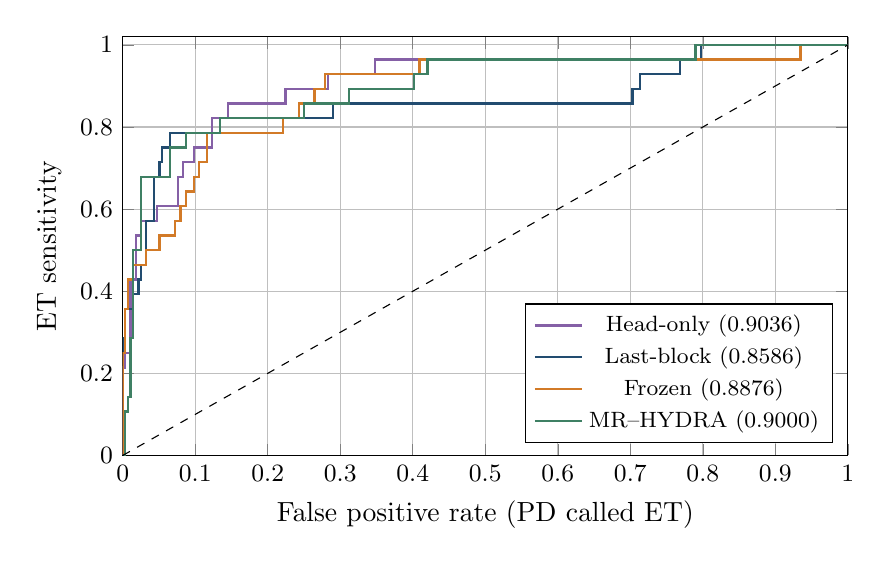
\begin{tikzpicture}
\begin{axis}[width=.89\linewidth,height=6.9cm,xmin=0,xmax=1,ymin=0,ymax=1.02,
 xlabel={False positive rate (PD called ET)},ylabel={ET sensitivity},grid=major,
 legend style={at={(.98,.03)},anchor=south east,font=\footnotesize,fill=white},
 tick label style={font=\small}]
\addplot[purpleplot,thick] coordinates {(0.0000000,0.0000000) (0.0000000,0.0357143) (0.0000000,0.0714286) (0.0000000,0.1071429) (0.0000000,0.1428571) (0.0000000,0.1785714) (0.0000000,0.2142857) (0.0036232,0.2142857) (0.0036232,0.2500000) (0.0072464,0.2500000) (0.0108696,0.2500000) (0.0108696,0.2857143) (0.0108696,0.3214286) (0.0108696,0.3571429) (0.0108696,0.3928571) (0.0108696,0.4285714) (0.0144928,0.4285714) (0.0181159,0.4285714) (0.0181159,0.4642857) (0.0181159,0.5000000) (0.0181159,0.5357143) (0.0217391,0.5357143) (0.0253623,0.5357143) (0.0253623,0.5714286) (0.0289855,0.5714286) (0.0326087,0.5714286) (0.0362319,0.5714286) (0.0398551,0.5714286) (0.0434783,0.5714286) (0.0471014,0.5714286) (0.0471014,0.6071429) (0.0507246,0.6071429) (0.0543478,0.6071429) (0.0579710,0.6071429) (0.0615942,0.6071429) (0.0652174,0.6071429) (0.0688406,0.6071429) (0.0724638,0.6071429) (0.0760870,0.6071429) (0.0760870,0.6428571) (0.0760870,0.6785714) (0.0797101,0.6785714) (0.0833333,0.6785714) (0.0833333,0.7142857) (0.0869565,0.7142857) (0.0905797,0.7142857) (0.0942029,0.7142857) (0.0978261,0.7142857) (0.0978261,0.7500000) (0.1014493,0.7500000) (0.1050725,0.7500000) (0.1086957,0.7500000) (0.1123188,0.7500000) (0.1159420,0.7500000) (0.1195652,0.7500000) (0.1231884,0.7500000) (0.1231884,0.7857143) (0.1231884,0.8214286) (0.1268116,0.8214286) (0.1304348,0.8214286) (0.1340580,0.8214286) (0.1376812,0.8214286) (0.1413043,0.8214286) (0.1449275,0.8214286) (0.1449275,0.8571429) (0.1485507,0.8571429) (0.1521739,0.8571429) (0.1557971,0.8571429) (0.1594203,0.8571429) (0.1630435,0.8571429) (0.1666667,0.8571429) (0.1702899,0.8571429) (0.1739130,0.8571429) (0.1775362,0.8571429) (0.1811594,0.8571429) (0.1847826,0.8571429) (0.1884058,0.8571429) (0.1920290,0.8571429) (0.1956522,0.8571429) (0.1992754,0.8571429) (0.2028986,0.8571429) (0.2065217,0.8571429) (0.2101449,0.8571429) (0.2137681,0.8571429) (0.2173913,0.8571429) (0.2210145,0.8571429) (0.2246377,0.8571429) (0.2246377,0.8928571) (0.2282609,0.8928571) (0.2318841,0.8928571) (0.2355072,0.8928571) (0.2391304,0.8928571) (0.2427536,0.8928571) (0.2463768,0.8928571) (0.2500000,0.8928571) (0.2536232,0.8928571) (0.2572464,0.8928571) (0.2608696,0.8928571) (0.2644928,0.8928571) (0.2681159,0.8928571) (0.2717391,0.8928571) (0.2753623,0.8928571) (0.2789855,0.8928571) (0.2826087,0.8928571) (0.2826087,0.9285714) (0.2862319,0.9285714) (0.2898551,0.9285714) (0.2934783,0.9285714) (0.2971014,0.9285714) (0.3007246,0.9285714) (0.3043478,0.9285714) (0.3079710,0.9285714) (0.3115942,0.9285714) (0.3152174,0.9285714) (0.3188406,0.9285714) (0.3224638,0.9285714) (0.3260870,0.9285714) (0.3297101,0.9285714) (0.3333333,0.9285714) (0.3369565,0.9285714) (0.3405797,0.9285714) (0.3442029,0.9285714) (0.3478261,0.9285714) (0.3478261,0.9642857) (0.3514493,0.9642857) (0.3550725,0.9642857) (0.3586957,0.9642857) (0.3623188,0.9642857) (0.3659420,0.9642857) (0.3695652,0.9642857) (0.3731884,0.9642857) (0.3768116,0.9642857) (0.3804348,0.9642857) (0.3840580,0.9642857) (0.3876812,0.9642857) (0.3913043,0.9642857) (0.3949275,0.9642857) (0.3985507,0.9642857) (0.4021739,0.9642857) (0.4057971,0.9642857) (0.4094203,0.9642857) (0.4130435,0.9642857) (0.4166667,0.9642857) (0.4202899,0.9642857) (0.4239130,0.9642857) (0.4275362,0.9642857) (0.4311594,0.9642857) (0.4347826,0.9642857) (0.4384058,0.9642857) (0.4420290,0.9642857) (0.4456522,0.9642857) (0.4492754,0.9642857) (0.4528986,0.9642857) (0.4565217,0.9642857) (0.4601449,0.9642857) (0.4637681,0.9642857) (0.4673913,0.9642857) (0.4710145,0.9642857) (0.4746377,0.9642857) (0.4782609,0.9642857) (0.4818841,0.9642857) (0.4855072,0.9642857) (0.4891304,0.9642857) (0.4927536,0.9642857) (0.4963768,0.9642857) (0.5000000,0.9642857) (0.5036232,0.9642857) (0.5072464,0.9642857) (0.5108696,0.9642857) (0.5144928,0.9642857) (0.5181159,0.9642857) (0.5217391,0.9642857) (0.5253623,0.9642857) (0.5289855,0.9642857) (0.5326087,0.9642857) (0.5362319,0.9642857) (0.5398551,0.9642857) (0.5434783,0.9642857) (0.5471014,0.9642857) (0.5507246,0.9642857) (0.5543478,0.9642857) (0.5579710,0.9642857) (0.5615942,0.9642857) (0.5652174,0.9642857) (0.5688406,0.9642857) (0.5724638,0.9642857) (0.5760870,0.9642857) (0.5797101,0.9642857) (0.5833333,0.9642857) (0.5869565,0.9642857) (0.5905797,0.9642857) (0.5942029,0.9642857) (0.5978261,0.9642857) (0.6014493,0.9642857) (0.6050725,0.9642857) (0.6086957,0.9642857) (0.6123188,0.9642857) (0.6159420,0.9642857) (0.6195652,0.9642857) (0.6231884,0.9642857) (0.6268116,0.9642857) (0.6304348,0.9642857) (0.6340580,0.9642857) (0.6376812,0.9642857) (0.6413043,0.9642857) (0.6449275,0.9642857) (0.6485507,0.9642857) (0.6521739,0.9642857) (0.6557971,0.9642857) (0.6594203,0.9642857) (0.6630435,0.9642857) (0.6666667,0.9642857) (0.6702899,0.9642857) (0.6739130,0.9642857) (0.6775362,0.9642857) (0.6811594,0.9642857) (0.6847826,0.9642857) (0.6884058,0.9642857) (0.6920290,0.9642857) (0.6956522,0.9642857) (0.6992754,0.9642857) (0.7028986,0.9642857) (0.7065217,0.9642857) (0.7101449,0.9642857) (0.7137681,0.9642857) (0.7173913,0.9642857) (0.7210145,0.9642857) (0.7246377,0.9642857) (0.7282609,0.9642857) (0.7318841,0.9642857) (0.7355072,0.9642857) (0.7391304,0.9642857) (0.7427536,0.9642857) (0.7463768,0.9642857) (0.7500000,0.9642857) (0.7536232,0.9642857) (0.7572464,0.9642857) (0.7608696,0.9642857) (0.7644928,0.9642857) (0.7681159,0.9642857) (0.7717391,0.9642857) (0.7753623,0.9642857) (0.7789855,0.9642857) (0.7826087,0.9642857) (0.7862319,0.9642857) (0.7898551,0.9642857) (0.7934783,0.9642857) (0.7971014,0.9642857) (0.8007246,0.9642857) (0.8043478,0.9642857) (0.8079710,0.9642857) (0.8115942,0.9642857) (0.8152174,0.9642857) (0.8188406,0.9642857) (0.8224638,0.9642857) (0.8260870,0.9642857) (0.8297101,0.9642857) (0.8333333,0.9642857) (0.8369565,0.9642857) (0.8405797,0.9642857) (0.8442029,0.9642857) (0.8478261,0.9642857) (0.8514493,0.9642857) (0.8550725,0.9642857) (0.8586957,0.9642857) (0.8623188,0.9642857) (0.8659420,0.9642857) (0.8695652,0.9642857) (0.8731884,0.9642857) (0.8768116,0.9642857) (0.8804348,0.9642857) (0.8840580,0.9642857) (0.8876812,0.9642857) (0.8913043,0.9642857) (0.8949275,0.9642857) (0.8985507,0.9642857) (0.9021739,0.9642857) (0.9057971,0.9642857) (0.9094203,0.9642857) (0.9130435,0.9642857) (0.9166667,0.9642857) (0.9202899,0.9642857) (0.9239130,0.9642857) (0.9275362,0.9642857) (0.9311594,0.9642857) (0.9347826,0.9642857) (0.9347826,1.0000000) (0.9384058,1.0000000) (0.9420290,1.0000000) (0.9456522,1.0000000) (0.9492754,1.0000000) (0.9528986,1.0000000) (0.9565217,1.0000000) (0.9601449,1.0000000) (0.9637681,1.0000000) (0.9673913,1.0000000) (0.9710145,1.0000000) (0.9746377,1.0000000) (0.9782609,1.0000000) (0.9818841,1.0000000) (0.9855072,1.0000000) (0.9891304,1.0000000) (0.9927536,1.0000000) (0.9963768,1.0000000) (1.0000000,1.0000000)};\addlegendentry{Head-only (0.9036)}
\addplot[navy,thick] coordinates {(0.0000000,0.0000000) (0.0000000,0.0357143) (0.0000000,0.0714286) (0.0000000,0.1071429) (0.0000000,0.1428571) (0.0000000,0.1785714) (0.0000000,0.2142857) (0.0000000,0.2500000) (0.0000000,0.2857143) (0.0036232,0.2857143) (0.0036232,0.3214286) (0.0036232,0.3571429) (0.0072464,0.3571429) (0.0108696,0.3571429) (0.0144928,0.3571429) (0.0144928,0.3928571) (0.0181159,0.3928571) (0.0217391,0.3928571) (0.0217391,0.4285714) (0.0253623,0.4285714) (0.0253623,0.4642857) (0.0289855,0.4642857) (0.0326087,0.4642857) (0.0326087,0.5000000) (0.0326087,0.5357143) (0.0326087,0.5714286) (0.0362319,0.5714286) (0.0398551,0.5714286) (0.0434783,0.5714286) (0.0434783,0.6071429) (0.0434783,0.6428571) (0.0434783,0.6785714) (0.0471014,0.6785714) (0.0507246,0.6785714) (0.0507246,0.7142857) (0.0543478,0.7142857) (0.0543478,0.7500000) (0.0579710,0.7500000) (0.0615942,0.7500000) (0.0652174,0.7500000) (0.0652174,0.7857143) (0.0688406,0.7857143) (0.0724638,0.7857143) (0.0760870,0.7857143) (0.0797101,0.7857143) (0.0833333,0.7857143) (0.0869565,0.7857143) (0.0905797,0.7857143) (0.0942029,0.7857143) (0.0978261,0.7857143) (0.1014493,0.7857143) (0.1050725,0.7857143) (0.1086957,0.7857143) (0.1123188,0.7857143) (0.1159420,0.7857143) (0.1195652,0.7857143) (0.1231884,0.7857143) (0.1268116,0.7857143) (0.1304348,0.7857143) (0.1340580,0.7857143) (0.1376812,0.7857143) (0.1413043,0.7857143) (0.1449275,0.7857143) (0.1485507,0.7857143) (0.1521739,0.7857143) (0.1557971,0.7857143) (0.1594203,0.7857143) (0.1630435,0.7857143) (0.1666667,0.7857143) (0.1702899,0.7857143) (0.1739130,0.7857143) (0.1775362,0.7857143) (0.1811594,0.7857143) (0.1847826,0.7857143) (0.1884058,0.7857143) (0.1920290,0.7857143) (0.1956522,0.7857143) (0.1992754,0.7857143) (0.2028986,0.7857143) (0.2065217,0.7857143) (0.2101449,0.7857143) (0.2137681,0.7857143) (0.2173913,0.7857143) (0.2210145,0.7857143) (0.2210145,0.8214286) (0.2246377,0.8214286) (0.2282609,0.8214286) (0.2318841,0.8214286) (0.2355072,0.8214286) (0.2391304,0.8214286) (0.2427536,0.8214286) (0.2463768,0.8214286) (0.2500000,0.8214286) (0.2536232,0.8214286) (0.2572464,0.8214286) (0.2608696,0.8214286) (0.2644928,0.8214286) (0.2681159,0.8214286) (0.2717391,0.8214286) (0.2753623,0.8214286) (0.2789855,0.8214286) (0.2826087,0.8214286) (0.2862319,0.8214286) (0.2898551,0.8214286) (0.2898551,0.8571429) (0.2934783,0.8571429) (0.2971014,0.8571429) (0.3007246,0.8571429) (0.3043478,0.8571429) (0.3079710,0.8571429) (0.3115942,0.8571429) (0.3152174,0.8571429) (0.3188406,0.8571429) (0.3224638,0.8571429) (0.3260870,0.8571429) (0.3297101,0.8571429) (0.3333333,0.8571429) (0.3369565,0.8571429) (0.3405797,0.8571429) (0.3442029,0.8571429) (0.3478261,0.8571429) (0.3514493,0.8571429) (0.3550725,0.8571429) (0.3586957,0.8571429) (0.3623188,0.8571429) (0.3659420,0.8571429) (0.3695652,0.8571429) (0.3731884,0.8571429) (0.3768116,0.8571429) (0.3804348,0.8571429) (0.3840580,0.8571429) (0.3876812,0.8571429) (0.3913043,0.8571429) (0.3949275,0.8571429) (0.3985507,0.8571429) (0.4021739,0.8571429) (0.4057971,0.8571429) (0.4094203,0.8571429) (0.4130435,0.8571429) (0.4166667,0.8571429) (0.4202899,0.8571429) (0.4239130,0.8571429) (0.4275362,0.8571429) (0.4311594,0.8571429) (0.4347826,0.8571429) (0.4384058,0.8571429) (0.4420290,0.8571429) (0.4456522,0.8571429) (0.4492754,0.8571429) (0.4528986,0.8571429) (0.4565217,0.8571429) (0.4601449,0.8571429) (0.4637681,0.8571429) (0.4673913,0.8571429) (0.4710145,0.8571429) (0.4746377,0.8571429) (0.4782609,0.8571429) (0.4818841,0.8571429) (0.4855072,0.8571429) (0.4891304,0.8571429) (0.4927536,0.8571429) (0.4963768,0.8571429) (0.5000000,0.8571429) (0.5036232,0.8571429) (0.5072464,0.8571429) (0.5108696,0.8571429) (0.5144928,0.8571429) (0.5181159,0.8571429) (0.5217391,0.8571429) (0.5253623,0.8571429) (0.5289855,0.8571429) (0.5326087,0.8571429) (0.5362319,0.8571429) (0.5398551,0.8571429) (0.5434783,0.8571429) (0.5471014,0.8571429) (0.5507246,0.8571429) (0.5543478,0.8571429) (0.5579710,0.8571429) (0.5615942,0.8571429) (0.5652174,0.8571429) (0.5688406,0.8571429) (0.5724638,0.8571429) (0.5760870,0.8571429) (0.5797101,0.8571429) (0.5833333,0.8571429) (0.5869565,0.8571429) (0.5905797,0.8571429) (0.5942029,0.8571429) (0.5978261,0.8571429) (0.6014493,0.8571429) (0.6050725,0.8571429) (0.6086957,0.8571429) (0.6123188,0.8571429) (0.6159420,0.8571429) (0.6195652,0.8571429) (0.6231884,0.8571429) (0.6268116,0.8571429) (0.6304348,0.8571429) (0.6340580,0.8571429) (0.6376812,0.8571429) (0.6413043,0.8571429) (0.6449275,0.8571429) (0.6485507,0.8571429) (0.6521739,0.8571429) (0.6557971,0.8571429) (0.6594203,0.8571429) (0.6630435,0.8571429) (0.6666667,0.8571429) (0.6702899,0.8571429) (0.6739130,0.8571429) (0.6775362,0.8571429) (0.6811594,0.8571429) (0.6847826,0.8571429) (0.6884058,0.8571429) (0.6920290,0.8571429) (0.6956522,0.8571429) (0.6992754,0.8571429) (0.7028986,0.8571429) (0.7028986,0.8928571) (0.7065217,0.8928571) (0.7101449,0.8928571) (0.7137681,0.8928571) (0.7137681,0.9285714) (0.7173913,0.9285714) (0.7210145,0.9285714) (0.7246377,0.9285714) (0.7282609,0.9285714) (0.7318841,0.9285714) (0.7355072,0.9285714) (0.7391304,0.9285714) (0.7427536,0.9285714) (0.7463768,0.9285714) (0.7500000,0.9285714) (0.7536232,0.9285714) (0.7572464,0.9285714) (0.7608696,0.9285714) (0.7644928,0.9285714) (0.7681159,0.9285714) (0.7681159,0.9642857) (0.7717391,0.9642857) (0.7753623,0.9642857) (0.7789855,0.9642857) (0.7826087,0.9642857) (0.7862319,0.9642857) (0.7898551,0.9642857) (0.7934783,0.9642857) (0.7971014,0.9642857) (0.7971014,1.0000000) (0.8007246,1.0000000) (0.8043478,1.0000000) (0.8079710,1.0000000) (0.8115942,1.0000000) (0.8152174,1.0000000) (0.8188406,1.0000000) (0.8224638,1.0000000) (0.8260870,1.0000000) (0.8297101,1.0000000) (0.8333333,1.0000000) (0.8369565,1.0000000) (0.8405797,1.0000000) (0.8442029,1.0000000) (0.8478261,1.0000000) (0.8514493,1.0000000) (0.8550725,1.0000000) (0.8586957,1.0000000) (0.8623188,1.0000000) (0.8659420,1.0000000) (0.8695652,1.0000000) (0.8731884,1.0000000) (0.8768116,1.0000000) (0.8804348,1.0000000) (0.8840580,1.0000000) (0.8876812,1.0000000) (0.8913043,1.0000000) (0.8949275,1.0000000) (0.8985507,1.0000000) (0.9021739,1.0000000) (0.9057971,1.0000000) (0.9094203,1.0000000) (0.9130435,1.0000000) (0.9166667,1.0000000) (0.9202899,1.0000000) (0.9239130,1.0000000) (0.9275362,1.0000000) (0.9311594,1.0000000) (0.9347826,1.0000000) (0.9384058,1.0000000) (0.9420290,1.0000000) (0.9456522,1.0000000) (0.9492754,1.0000000) (0.9528986,1.0000000) (0.9565217,1.0000000) (0.9601449,1.0000000) (0.9637681,1.0000000) (0.9673913,1.0000000) (0.9710145,1.0000000) (0.9746377,1.0000000) (0.9782609,1.0000000) (0.9818841,1.0000000) (0.9855072,1.0000000) (0.9891304,1.0000000) (0.9927536,1.0000000) (0.9963768,1.0000000) (1.0000000,1.0000000)};\addlegendentry{Last-block (0.8586)}
\addplot[orangeplot,thick] coordinates {(0.0000000,0.0000000) (0.0000000,0.0357143) (0.0000000,0.0714286) (0.0000000,0.1071429) (0.0000000,0.1428571) (0.0000000,0.1785714) (0.0000000,0.2142857) (0.0000000,0.2500000) (0.0036232,0.2500000) (0.0036232,0.2857143) (0.0036232,0.3214286) (0.0036232,0.3571429) (0.0072464,0.3571429) (0.0072464,0.3928571) (0.0072464,0.4285714) (0.0108696,0.4285714) (0.0144928,0.4285714) (0.0144928,0.4642857) (0.0181159,0.4642857) (0.0217391,0.4642857) (0.0253623,0.4642857) (0.0289855,0.4642857) (0.0326087,0.4642857) (0.0326087,0.5000000) (0.0362319,0.5000000) (0.0398551,0.5000000) (0.0434783,0.5000000) (0.0471014,0.5000000) (0.0507246,0.5000000) (0.0507246,0.5357143) (0.0543478,0.5357143) (0.0579710,0.5357143) (0.0615942,0.5357143) (0.0652174,0.5357143) (0.0688406,0.5357143) (0.0724638,0.5357143) (0.0724638,0.5714286) (0.0760870,0.5714286) (0.0797101,0.5714286) (0.0797101,0.6071429) (0.0833333,0.6071429) (0.0869565,0.6071429) (0.0869565,0.6428571) (0.0905797,0.6428571) (0.0942029,0.6428571) (0.0978261,0.6428571) (0.0978261,0.6785714) (0.1014493,0.6785714) (0.1050725,0.6785714) (0.1050725,0.7142857) (0.1086957,0.7142857) (0.1123188,0.7142857) (0.1159420,0.7142857) (0.1159420,0.7500000) (0.1159420,0.7857143) (0.1195652,0.7857143) (0.1231884,0.7857143) (0.1268116,0.7857143) (0.1304348,0.7857143) (0.1340580,0.7857143) (0.1376812,0.7857143) (0.1413043,0.7857143) (0.1449275,0.7857143) (0.1485507,0.7857143) (0.1521739,0.7857143) (0.1557971,0.7857143) (0.1594203,0.7857143) (0.1630435,0.7857143) (0.1666667,0.7857143) (0.1702899,0.7857143) (0.1739130,0.7857143) (0.1775362,0.7857143) (0.1811594,0.7857143) (0.1847826,0.7857143) (0.1884058,0.7857143) (0.1920290,0.7857143) (0.1956522,0.7857143) (0.1992754,0.7857143) (0.2028986,0.7857143) (0.2065217,0.7857143) (0.2101449,0.7857143) (0.2137681,0.7857143) (0.2173913,0.7857143) (0.2210145,0.7857143) (0.2210145,0.8214286) (0.2246377,0.8214286) (0.2282609,0.8214286) (0.2318841,0.8214286) (0.2355072,0.8214286) (0.2391304,0.8214286) (0.2427536,0.8214286) (0.2427536,0.8571429) (0.2463768,0.8571429) (0.2500000,0.8571429) (0.2536232,0.8571429) (0.2572464,0.8571429) (0.2608696,0.8571429) (0.2644928,0.8571429) (0.2644928,0.8928571) (0.2681159,0.8928571) (0.2717391,0.8928571) (0.2753623,0.8928571) (0.2789855,0.8928571) (0.2789855,0.9285714) (0.2826087,0.9285714) (0.2862319,0.9285714) (0.2898551,0.9285714) (0.2934783,0.9285714) (0.2971014,0.9285714) (0.3007246,0.9285714) (0.3043478,0.9285714) (0.3079710,0.9285714) (0.3115942,0.9285714) (0.3152174,0.9285714) (0.3188406,0.9285714) (0.3224638,0.9285714) (0.3260870,0.9285714) (0.3297101,0.9285714) (0.3333333,0.9285714) (0.3369565,0.9285714) (0.3405797,0.9285714) (0.3442029,0.9285714) (0.3478261,0.9285714) (0.3514493,0.9285714) (0.3550725,0.9285714) (0.3586957,0.9285714) (0.3623188,0.9285714) (0.3659420,0.9285714) (0.3695652,0.9285714) (0.3731884,0.9285714) (0.3768116,0.9285714) (0.3804348,0.9285714) (0.3840580,0.9285714) (0.3876812,0.9285714) (0.3913043,0.9285714) (0.3949275,0.9285714) (0.3985507,0.9285714) (0.4021739,0.9285714) (0.4057971,0.9285714) (0.4094203,0.9285714) (0.4094203,0.9642857) (0.4130435,0.9642857) (0.4166667,0.9642857) (0.4202899,0.9642857) (0.4239130,0.9642857) (0.4275362,0.9642857) (0.4311594,0.9642857) (0.4347826,0.9642857) (0.4384058,0.9642857) (0.4420290,0.9642857) (0.4456522,0.9642857) (0.4492754,0.9642857) (0.4528986,0.9642857) (0.4565217,0.9642857) (0.4601449,0.9642857) (0.4637681,0.9642857) (0.4673913,0.9642857) (0.4710145,0.9642857) (0.4746377,0.9642857) (0.4782609,0.9642857) (0.4818841,0.9642857) (0.4855072,0.9642857) (0.4891304,0.9642857) (0.4927536,0.9642857) (0.4963768,0.9642857) (0.5000000,0.9642857) (0.5036232,0.9642857) (0.5072464,0.9642857) (0.5108696,0.9642857) (0.5144928,0.9642857) (0.5181159,0.9642857) (0.5217391,0.9642857) (0.5253623,0.9642857) (0.5289855,0.9642857) (0.5326087,0.9642857) (0.5362319,0.9642857) (0.5398551,0.9642857) (0.5434783,0.9642857) (0.5471014,0.9642857) (0.5507246,0.9642857) (0.5543478,0.9642857) (0.5579710,0.9642857) (0.5615942,0.9642857) (0.5652174,0.9642857) (0.5688406,0.9642857) (0.5724638,0.9642857) (0.5760870,0.9642857) (0.5797101,0.9642857) (0.5833333,0.9642857) (0.5869565,0.9642857) (0.5905797,0.9642857) (0.5942029,0.9642857) (0.5978261,0.9642857) (0.6014493,0.9642857) (0.6050725,0.9642857) (0.6086957,0.9642857) (0.6123188,0.9642857) (0.6159420,0.9642857) (0.6195652,0.9642857) (0.6231884,0.9642857) (0.6268116,0.9642857) (0.6304348,0.9642857) (0.6340580,0.9642857) (0.6376812,0.9642857) (0.6413043,0.9642857) (0.6449275,0.9642857) (0.6485507,0.9642857) (0.6521739,0.9642857) (0.6557971,0.9642857) (0.6594203,0.9642857) (0.6630435,0.9642857) (0.6666667,0.9642857) (0.6702899,0.9642857) (0.6739130,0.9642857) (0.6775362,0.9642857) (0.6811594,0.9642857) (0.6847826,0.9642857) (0.6884058,0.9642857) (0.6920290,0.9642857) (0.6956522,0.9642857) (0.6992754,0.9642857) (0.7028986,0.9642857) (0.7065217,0.9642857) (0.7101449,0.9642857) (0.7137681,0.9642857) (0.7173913,0.9642857) (0.7210145,0.9642857) (0.7246377,0.9642857) (0.7282609,0.9642857) (0.7318841,0.9642857) (0.7355072,0.9642857) (0.7391304,0.9642857) (0.7427536,0.9642857) (0.7463768,0.9642857) (0.7500000,0.9642857) (0.7536232,0.9642857) (0.7572464,0.9642857) (0.7608696,0.9642857) (0.7644928,0.9642857) (0.7681159,0.9642857) (0.7717391,0.9642857) (0.7753623,0.9642857) (0.7789855,0.9642857) (0.7826087,0.9642857) (0.7862319,0.9642857) (0.7898551,0.9642857) (0.7934783,0.9642857) (0.7971014,0.9642857) (0.8007246,0.9642857) (0.8043478,0.9642857) (0.8079710,0.9642857) (0.8115942,0.9642857) (0.8152174,0.9642857) (0.8188406,0.9642857) (0.8224638,0.9642857) (0.8260870,0.9642857) (0.8297101,0.9642857) (0.8333333,0.9642857) (0.8369565,0.9642857) (0.8405797,0.9642857) (0.8442029,0.9642857) (0.8478261,0.9642857) (0.8514493,0.9642857) (0.8550725,0.9642857) (0.8586957,0.9642857) (0.8623188,0.9642857) (0.8659420,0.9642857) (0.8695652,0.9642857) (0.8731884,0.9642857) (0.8768116,0.9642857) (0.8804348,0.9642857) (0.8840580,0.9642857) (0.8876812,0.9642857) (0.8913043,0.9642857) (0.8949275,0.9642857) (0.8985507,0.9642857) (0.9021739,0.9642857) (0.9057971,0.9642857) (0.9094203,0.9642857) (0.9130435,0.9642857) (0.9166667,0.9642857) (0.9202899,0.9642857) (0.9239130,0.9642857) (0.9275362,0.9642857) (0.9311594,0.9642857) (0.9347826,0.9642857) (0.9347826,1.0000000) (0.9384058,1.0000000) (0.9420290,1.0000000) (0.9456522,1.0000000) (0.9492754,1.0000000) (0.9528986,1.0000000) (0.9565217,1.0000000) (0.9601449,1.0000000) (0.9637681,1.0000000) (0.9673913,1.0000000) (0.9710145,1.0000000) (0.9746377,1.0000000) (0.9782609,1.0000000) (0.9818841,1.0000000) (0.9855072,1.0000000) (0.9891304,1.0000000) (0.9927536,1.0000000) (0.9963768,1.0000000) (1.0000000,1.0000000)};\addlegendentry{Frozen (0.8876)}
\addplot[greenplot,thick] coordinates {(0.0000000,0.0000000) (0.0036232,0.0000000) (0.0036232,0.0357143) (0.0036232,0.0714286) (0.0036232,0.1071429) (0.0072464,0.1071429) (0.0072464,0.1428571) (0.0108696,0.1428571) (0.0108696,0.1785714) (0.0108696,0.2142857) (0.0108696,0.2500000) (0.0108696,0.2857143) (0.0144928,0.2857143) (0.0144928,0.3214286) (0.0144928,0.3571429) (0.0144928,0.3928571) (0.0144928,0.4285714) (0.0144928,0.4642857) (0.0144928,0.5000000) (0.0181159,0.5000000) (0.0217391,0.5000000) (0.0253623,0.5000000) (0.0253623,0.5357143) (0.0253623,0.5714286) (0.0253623,0.6071429) (0.0253623,0.6428571) (0.0253623,0.6785714) (0.0289855,0.6785714) (0.0326087,0.6785714) (0.0362319,0.6785714) (0.0398551,0.6785714) (0.0434783,0.6785714) (0.0471014,0.6785714) (0.0507246,0.6785714) (0.0543478,0.6785714) (0.0579710,0.6785714) (0.0615942,0.6785714) (0.0652174,0.6785714) (0.0652174,0.7142857) (0.0652174,0.7500000) (0.0688406,0.7500000) (0.0724638,0.7500000) (0.0760870,0.7500000) (0.0797101,0.7500000) (0.0833333,0.7500000) (0.0869565,0.7500000) (0.0869565,0.7857143) (0.0905797,0.7857143) (0.0942029,0.7857143) (0.0978261,0.7857143) (0.1014493,0.7857143) (0.1050725,0.7857143) (0.1086957,0.7857143) (0.1123188,0.7857143) (0.1159420,0.7857143) (0.1195652,0.7857143) (0.1231884,0.7857143) (0.1268116,0.7857143) (0.1304348,0.7857143) (0.1340580,0.7857143) (0.1340580,0.8214286) (0.1376812,0.8214286) (0.1413043,0.8214286) (0.1449275,0.8214286) (0.1485507,0.8214286) (0.1521739,0.8214286) (0.1557971,0.8214286) (0.1594203,0.8214286) (0.1630435,0.8214286) (0.1666667,0.8214286) (0.1702899,0.8214286) (0.1739130,0.8214286) (0.1775362,0.8214286) (0.1811594,0.8214286) (0.1847826,0.8214286) (0.1884058,0.8214286) (0.1920290,0.8214286) (0.1956522,0.8214286) (0.1992754,0.8214286) (0.2028986,0.8214286) (0.2065217,0.8214286) (0.2101449,0.8214286) (0.2137681,0.8214286) (0.2173913,0.8214286) (0.2210145,0.8214286) (0.2246377,0.8214286) (0.2282609,0.8214286) (0.2318841,0.8214286) (0.2355072,0.8214286) (0.2391304,0.8214286) (0.2427536,0.8214286) (0.2463768,0.8214286) (0.2500000,0.8214286) (0.2500000,0.8571429) (0.2536232,0.8571429) (0.2572464,0.8571429) (0.2608696,0.8571429) (0.2644928,0.8571429) (0.2681159,0.8571429) (0.2717391,0.8571429) (0.2753623,0.8571429) (0.2789855,0.8571429) (0.2826087,0.8571429) (0.2862319,0.8571429) (0.2898551,0.8571429) (0.2934783,0.8571429) (0.2971014,0.8571429) (0.3007246,0.8571429) (0.3043478,0.8571429) (0.3079710,0.8571429) (0.3115942,0.8571429) (0.3115942,0.8928571) (0.3152174,0.8928571) (0.3188406,0.8928571) (0.3224638,0.8928571) (0.3260870,0.8928571) (0.3297101,0.8928571) (0.3333333,0.8928571) (0.3369565,0.8928571) (0.3405797,0.8928571) (0.3442029,0.8928571) (0.3478261,0.8928571) (0.3514493,0.8928571) (0.3550725,0.8928571) (0.3586957,0.8928571) (0.3623188,0.8928571) (0.3659420,0.8928571) (0.3695652,0.8928571) (0.3731884,0.8928571) (0.3768116,0.8928571) (0.3804348,0.8928571) (0.3840580,0.8928571) (0.3876812,0.8928571) (0.3913043,0.8928571) (0.3949275,0.8928571) (0.3985507,0.8928571) (0.4021739,0.8928571) (0.4021739,0.9285714) (0.4057971,0.9285714) (0.4094203,0.9285714) (0.4130435,0.9285714) (0.4166667,0.9285714) (0.4202899,0.9285714) (0.4202899,0.9642857) (0.4239130,0.9642857) (0.4275362,0.9642857) (0.4311594,0.9642857) (0.4347826,0.9642857) (0.4384058,0.9642857) (0.4420290,0.9642857) (0.4456522,0.9642857) (0.4492754,0.9642857) (0.4528986,0.9642857) (0.4565217,0.9642857) (0.4601449,0.9642857) (0.4637681,0.9642857) (0.4673913,0.9642857) (0.4710145,0.9642857) (0.4746377,0.9642857) (0.4782609,0.9642857) (0.4818841,0.9642857) (0.4855072,0.9642857) (0.4891304,0.9642857) (0.4927536,0.9642857) (0.4963768,0.9642857) (0.5000000,0.9642857) (0.5036232,0.9642857) (0.5072464,0.9642857) (0.5108696,0.9642857) (0.5144928,0.9642857) (0.5181159,0.9642857) (0.5217391,0.9642857) (0.5253623,0.9642857) (0.5289855,0.9642857) (0.5326087,0.9642857) (0.5362319,0.9642857) (0.5398551,0.9642857) (0.5434783,0.9642857) (0.5471014,0.9642857) (0.5507246,0.9642857) (0.5543478,0.9642857) (0.5579710,0.9642857) (0.5615942,0.9642857) (0.5652174,0.9642857) (0.5688406,0.9642857) (0.5724638,0.9642857) (0.5760870,0.9642857) (0.5797101,0.9642857) (0.5833333,0.9642857) (0.5869565,0.9642857) (0.5905797,0.9642857) (0.5942029,0.9642857) (0.5978261,0.9642857) (0.6014493,0.9642857) (0.6050725,0.9642857) (0.6086957,0.9642857) (0.6123188,0.9642857) (0.6159420,0.9642857) (0.6195652,0.9642857) (0.6231884,0.9642857) (0.6268116,0.9642857) (0.6304348,0.9642857) (0.6340580,0.9642857) (0.6376812,0.9642857) (0.6413043,0.9642857) (0.6449275,0.9642857) (0.6485507,0.9642857) (0.6521739,0.9642857) (0.6557971,0.9642857) (0.6594203,0.9642857) (0.6630435,0.9642857) (0.6666667,0.9642857) (0.6702899,0.9642857) (0.6739130,0.9642857) (0.6775362,0.9642857) (0.6811594,0.9642857) (0.6847826,0.9642857) (0.6884058,0.9642857) (0.6920290,0.9642857) (0.6956522,0.9642857) (0.6992754,0.9642857) (0.7028986,0.9642857) (0.7065217,0.9642857) (0.7101449,0.9642857) (0.7137681,0.9642857) (0.7173913,0.9642857) (0.7210145,0.9642857) (0.7246377,0.9642857) (0.7282609,0.9642857) (0.7318841,0.9642857) (0.7355072,0.9642857) (0.7391304,0.9642857) (0.7427536,0.9642857) (0.7463768,0.9642857) (0.7500000,0.9642857) (0.7536232,0.9642857) (0.7572464,0.9642857) (0.7608696,0.9642857) (0.7644928,0.9642857) (0.7681159,0.9642857) (0.7717391,0.9642857) (0.7753623,0.9642857) (0.7789855,0.9642857) (0.7826087,0.9642857) (0.7862319,0.9642857) (0.7898551,0.9642857) (0.7898551,1.0000000) (0.7934783,1.0000000) (0.7971014,1.0000000) (0.8007246,1.0000000) (0.8043478,1.0000000) (0.8079710,1.0000000) (0.8115942,1.0000000) (0.8152174,1.0000000) (0.8188406,1.0000000) (0.8224638,1.0000000) (0.8260870,1.0000000) (0.8297101,1.0000000) (0.8333333,1.0000000) (0.8369565,1.0000000) (0.8405797,1.0000000) (0.8442029,1.0000000) (0.8478261,1.0000000) (0.8514493,1.0000000) (0.8550725,1.0000000) (0.8586957,1.0000000) (0.8623188,1.0000000) (0.8659420,1.0000000) (0.8695652,1.0000000) (0.8731884,1.0000000) (0.8768116,1.0000000) (0.8804348,1.0000000) (0.8840580,1.0000000) (0.8876812,1.0000000) (0.8913043,1.0000000) (0.8949275,1.0000000) (0.8985507,1.0000000) (0.9021739,1.0000000) (0.9057971,1.0000000) (0.9094203,1.0000000) (0.9130435,1.0000000) (0.9166667,1.0000000) (0.9202899,1.0000000) (0.9239130,1.0000000) (0.9275362,1.0000000) (0.9311594,1.0000000) (0.9347826,1.0000000) (0.9384058,1.0000000) (0.9420290,1.0000000) (0.9456522,1.0000000) (0.9492754,1.0000000) (0.9528986,1.0000000) (0.9565217,1.0000000) (0.9601449,1.0000000) (0.9637681,1.0000000) (0.9673913,1.0000000) (0.9710145,1.0000000) (0.9746377,1.0000000) (0.9782609,1.0000000) (0.9818841,1.0000000) (0.9855072,1.0000000) (0.9891304,1.0000000) (0.9927536,1.0000000) (0.9963768,1.0000000) (1.0000000,1.0000000)};\addlegendentry{MR--HYDRA (0.9000)}
\addplot[black,dashed] coordinates {(0,0)(1,1)};
\end{axis}\end{tikzpicture}
\caption{같은 외부 예측의 ROC 곡선. Last-block은 head-only보다 PR-AUC가 높고 pooled AUROC는 낮다.}
\end{figure}
\clearpage

\subsection{fold별 성능과 점수 척도}
\begin{table}[H]\centering\small\setlength{\tabcolsep}{4pt}
\caption{두 신경망 모드의 외부 fold별 결과. PD/ET는 정분류 수/해당 클래스 수다.}
\begin{tabular}{@{}lrrrrrrrr@{}}\toprule
모드 & Fold & PD & ET & BA(\%) & AUROC & PR-AUC & G-mean & MCC\\\midrule
Head-only & 1 & 43/56 & 4/5 & 78.39 & 0.9357 & 0.7968 & 0.7838 & 0.3474 \\
Head-only & 2 & 37/55 & 5/6 & 75.30 & 0.8212 & 0.6566 & 0.7487 & 0.3110 \\
Head-only & 3 & 43/55 & 6/6 & 89.09 & 0.9455 & 0.6587 & 0.8842 & 0.5105 \\
Head-only & 4 & 33/55 & 6/6 & 80.00 & 0.9909 & 0.9248 & 0.7746 & 0.3586 \\
Head-only & 5 & 38/55 & 5/5 & 84.55 & 0.8727 & 0.3169 & 0.8312 & 0.3963 \\
Last-block & 1 & 56/56 & 2/5 & 70.00 & 0.9571 & 0.8544 & 0.6325 & 0.6162 \\
Last-block & 2 & 52/55 & 2/6 & 63.94 & 0.8303 & 0.5945 & 0.5614 & 0.3027 \\
Last-block & 3 & 52/55 & 4/6 & 80.61 & 0.9242 & 0.5631 & 0.7939 & 0.5719 \\
Last-block & 4 & 53/55 & 6/6 & 98.18 & 0.9848 & 0.8663 & 0.9816 & 0.8501 \\
Last-block & 5 & 53/55 & 2/5 & 68.18 & 0.8509 & 0.5204 & 0.6208 & 0.4029 \\
\bottomrule\end{tabular}
\end{table}
\begin{table}[H]\centering\small\setlength{\tabcolsep}{4pt}
\caption{외부 fold 수치의 단순평균. BA SD는 fold 간 기술적 변동이며 표준오차가 아니다.}
\begin{tabular}{@{}lrrrrr@{}}\toprule
방법 & 평균 BA(\%) & BA SD(pp) & 평균 AUROC & 평균 PR-AUC & 평균 AP\\\midrule
Head-only & 81.47 & 5.41 & 0.9132 & 0.6708 & 0.6973 \\
Last-block & 76.18 & 13.74 & 0.9095 & 0.6797 & 0.6969 \\
Frozen MantisV2 & 70.79 & 6.73 & 0.8929 & 0.6538 & 0.6707 \\
MR--HYDRA & 66.94 & 6.08 & 0.9068 & 0.6396 & 0.6684 \\
\bottomrule\end{tabular}
\end{table}
Last-block의 평균 fold AUROC 0.9095는 pooled AUROC 0.8586과 다르다.
Head-only는 각각 0.9132와 0.9036이다.
외부 fold의 인코더, 정규화와 head는 서로 별도로 학습되므로
fold 간 logit의 위치와 척도가 다를 수 있다.
pooled AUROC/PR-AUC/AP에는 서로 다른 모델에서 나온 참가자 간 점수 비교가 포함된다.
평균 fold 지표는 각 모델 안에서 계산한 순위 지표를 평균한 것으로 다른 대상량이다.
이번 결과만으로 점수 척도 차이가 pooled 감소의 원인이라고 확정하지 않는다.

\begin{figure}[H]\centering
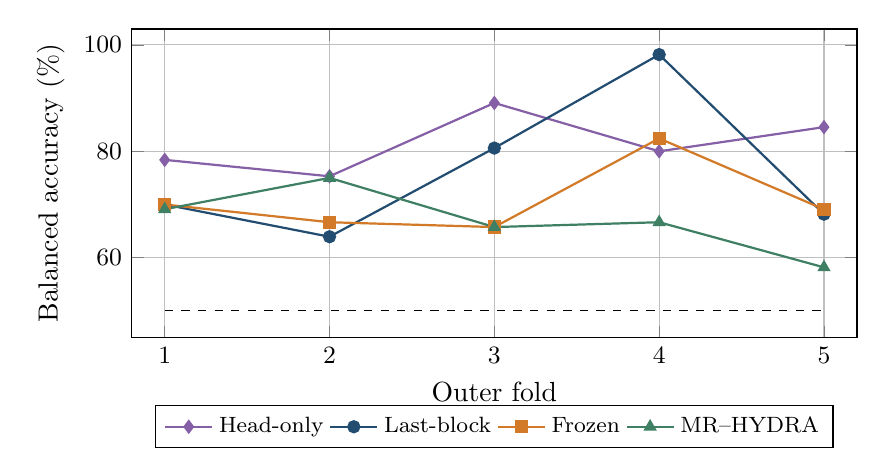
\begin{tikzpicture}
\begin{axis}[width=.89\linewidth,height=5.5cm,xmin=.8,xmax=5.2,ymin=45,ymax=103,
 xtick={1,2,3,4,5},xlabel={Outer fold},ylabel={Balanced accuracy (\%)},grid=major,
 legend style={at={(.5,-.22)},anchor=north,legend columns=4,font=\footnotesize},
 tick label style={font=\small}]
\addplot[purpleplot,mark=diamond*,thick] coordinates {(1.0000000,78.3928571) (2.0000000,75.3030303) (3.0000000,89.0909091) (4.0000000,80.0000000) (5.0000000,84.5454545)};\addlegendentry{Head-only}
\addplot[navy,mark=*,thick] coordinates {(1.0000000,70.0000000) (2.0000000,63.9393939) (3.0000000,80.6060606) (4.0000000,98.1818182) (5.0000000,68.1818182)};\addlegendentry{Last-block}
\addplot[orangeplot,mark=square*,thick] coordinates {(1.0000000,70.0000000) (2.0000000,66.6666667) (3.0000000,65.7575758) (4.0000000,82.4242424) (5.0000000,69.0909091)};\addlegendentry{Frozen}
\addplot[greenplot,mark=triangle*,thick] coordinates {(1.0000000,69.1071429) (2.0000000,75.0000000) (3.0000000,65.7575758) (4.0000000,66.6666667) (5.0000000,58.1818182)};\addlegendentry{MR--HYDRA}
\addplot[black,dashed] coordinates {(1,50)(5,50)};
\end{axis}\end{tikzpicture}
\caption{fold별 BA 변동. 각 평가 fold의 ET는 5--6명으로 재현율이 불연속적으로 변한다.}
\end{figure}
\clearpage

\section{Head-only 대조군과 Last-block 재실행}\label{sec:ablation}
\subsection{적응의 추가 효용과 운영점의 상충 관계}
Head-only와 last-block은 같은 사전학습 표현, head, 정규화, 가중 BCE,
head 학습률, dropout, 참가자 분할과 seed를 사용한다.
차이는 마지막 블록의 갱신 허용과 모드별 내부 선택 결과다.
Last-block에서 head-only를 뺀 pooled 변화는
\begin{align}
 \Delta\BA&=-4.81\ \mathrm{pp},&
 \Delta R_{\mathrm{ET}}&=-35.71\ \mathrm{pp},&
 \Delta R_{\mathrm{PD}}&=+26.09\ \mathrm{pp},\\
 \Delta\mathrm{PR}\text{-}\mathrm{AUC}&=+0.0073,&
 \Delta\mathrm{MCC}&=+0.1719.
\end{align}
Head-only가 검출한 ET 26명 중 10명을 last-block이 놓치는 대신,
head-only가 틀린 PD 82명 중 72명을 last-block이 바로잡는다.
따라서 인코더 적응은 이 구현에서 높은 ET 검출률을 유지한 채 전반적 성능을
일관되게 향상시키지 않았다. \textbf{주 지표 BA 개선 가설은 head-only 비교에서 지지되지 않는다.}
다만 last-block의 PD 특이도, ET 정밀도, MCC와 macro-F1은 더 높다.
PR-AUC 차이도 작아서 어떤 임상 운영점에서 우수한지를 이 값 하나로 정할 수 없다.

기존 고정 MantisV2+ridge와 비교하면 last-block의 BA는 5.87 pp,
ET 민감도는 14.29 pp 높고 PD 특이도는 2.54 pp 낮다.
PR-AUC는 0.6229에서 0.6463, AP는 0.6272에서 0.6505로 높아지지만
MCC는 0.5577에서 0.5534로 소폭 낮아진다.
Head-only 대조군의 추가로 \textbf{고정 ridge 대비 개선을 인코더 적응만의 성과로
돌릴 수 없다는 점}이 더 명확해졌다.

Head-only의 가장 높은 외부 BA를 보고 이 모드를 사후 선택하는 것은 별도의 선택 단계다.
그 선택까지 포함한 절차의 일반화 성능을 같은 외부 예측으로 다시 검증했다고 주장하지 않는다.
고정 epoch에서 순수한 적응 효과를 분리하는 추가 실험이나 임계값 재조정도 이번 분석에서 수행하지 않았다.

\subsection{완료 실행 기록과 재현성}
\begin{table}[H]\centering\footnotesize\setlength{\tabcolsep}{3pt}
\caption{세 완료 실행의 식별자와 시간. 시각은 2026년 KST, 경과 시간은 분 단위다.}
\label{tab:runs}
\begin{tabular}{@{}llllr@{}}\toprule
실행 & Run ID & 시작(MM-DD) & 종료(MM-DD) & 경과(분)\\\midrule
Head-only & \code{20261109T032315873662Z} & 11-09 12:23:15 & 11-09 13:16:43 & 53.46 \\
Last-block & \code{20261109T041659480074Z} & 11-09 13:16:59 & 11-09 16:53:47 & 216.13 \\
Last-block (old) & \code{20261108T145903609065Z} & 11-08 23:59:03 & 11-09 03:14:47 & 195.74 \\
\bottomrule\end{tabular}
\end{table}
Last-block의 주 결과는 가장 최근 실행을 사용한다. 이전 last-block과 새 실행은
304개 외부 예측, 내부 선택/탐색 결과, 재적합 손실 이력 및
저장 모델 6개의 모든 state tensor가 정확히 같았다.
최종 선택 분할과 초기 고정 특징 cache도 같았다.
이는 해당 환경과 seed에서의 재현 확인이며, 다른 seed나 장치에 대한 보장은 아니다.
두 last-block 실행은 \textbf{한 방법의 동일 분할 재실행}으로 취급하여
표의 방법 수, 참가자 수와 bootstrap 표본 크기에 중복 합산하지 않는다.

두 모드의 기록된 경과 시간은 탐색 전체의 시간이다.
Head-only는 24회, last-block은 42회 적합하며 역전파 범위도 다르다.
따라서 경과 시간을 동일 적합 횟수의 속도나 단일 참가자 추론 latency 비교로 해석하지 않는다.
\clearpage

\section{대응 비교와 불확실성}
\subsection{어떤 참가자의 예측이 달라졌는가}
\begin{table}[H]\centering\small\setlength{\tabcolsep}{4pt}
\caption{같은 참가자에서의 정오 분류 대응표. 두 방법의 참가자 대응을 유지하였다.}
\begin{tabular}{@{}lrrrr@{}}\toprule
비교군 / 실제 클래스 & 둘 다 정답 & Last만 정답 & 비교군만 정답 & 둘 다 오답\\\midrule
Head-only / PD & 194 & 72 & 0 & 10 \\
Head-only / ET & 16 & 0 & 10 & 2 \\
Frozen MantisV2 / PD & 265 & 1 & 8 & 2 \\
Frozen MantisV2 / ET & 12 & 4 & 0 & 12 \\
MR--HYDRA / PD & 264 & 2 & 8 & 2 \\
MR--HYDRA / ET & 9 & 7 & 1 & 11 \\
\bottomrule\end{tabular}
\end{table}
Last-block은 고정 MantisV2가 맞춘 ET 12명을 모두 유지하며 ET 4명을 추가로 맞췄다.
PD에서는 1명을 개선하고 8명을 새로 틀려 순수하게 7명 감소했다.
Head-only 비교에서는 PD 72명을 개선하고 ET 10명을 새로 놓쳤다.
이는 대응 예측의 관찰이며, 참가자의 임상적 개선이나 인과적 기전으로 해석하지 않는다.

\subsection{클래스별 대응 bootstrap}
불균형을 유지하기 위해 PD 276명과 ET 28명을 각각 복원추출한다.
하나의 bootstrap 표본에서 모든 방법에 \textbf{같은 참가자 인덱스}를 사용한다.
반복 수 $B=20{,}000$, NumPy seed 20261109로 설정하였다.
비교군 $m$과 last-block $F$에 대해
$d_i=\ind\{\widehat y_i^{F}=y_i\}-\ind\{\widehat y_i^m=y_i\}$라 하면
\begin{equation}
 \widehat\Delta_{\BA}^{*(b)}=
 \frac12\left[\frac1{276}\sum_{i\in I_{0}^{*(b)}}d_i+
 \frac1{28}\sum_{i\in I_{1}^{*(b)}}d_i\right]
\end{equation}
이며, $I_c^{*(b)}$는 클래스 $c$의 복원추출 다중집합이다.
2.5\%, 97.5\% 분위수를 조건부 구간으로 제시한다.
\begin{table}[H]\centering\small
\caption{Last-block에서 비교군을 뺀 BA 차이. 저장된 적합에 조건부인 percentile 구간이다.}
\begin{tabular}{@{}lrr@{}}\toprule
비교군 & BA 차이(pp) & 조건부 95\% 구간(pp)\\\midrule
Head-only & -4.81 & [-14.10, 4.14] \\
Frozen MantisV2 & 5.87 & [0.16, 13.02] \\
MR--HYDRA & 9.63 & [0.70, 18.92] \\
\bottomrule\end{tabular}
\end{table}
Head-only 대비 구간은 0을 포함한다. 두 기존 기준선 대비 구간은 이 재표집에서 0보다 크다.
어느 경우도 학습 절차의 통계적 우월성 또는 동등성 검정으로 해석하지 않는다.
모델을 다시 학습하지 않아 학습 표본 변화, 초기화, 하이퍼파라미터 선택 및
과거 결과를 본 뒤의 설계 변경에 따른 불확실성을 반영하지 않기 때문이다.
교차검증 학습 집합은 중첩되어 예측 오차가 완전히 독립적인 것도 아니다.
이 구간은 사전 등록한 우월성 검정이나 외부 검증의 신뢰구간이 아니다.

ET 한 명의 판정이 바뀌면 pooled ET 민감도는 $100/28=3.57$ pp,
PD 판정이 같을 때 BA는 $100/(2\cdot28)=1.79$ pp 바뀐다.
fold 내 ET가 5명 또는 6명이므로 한 명의 변화는 그 fold BA를 10 또는 8.33 pp 바꾼다.
외부 fold의 큰 변동과 ET 표본 수를 함께 고려해야 한다.
\clearpage

\section{학습 이력, 최종 모델과 해석의 한계}
\subsection{재적합 손실}
\begin{figure}[H]\centering
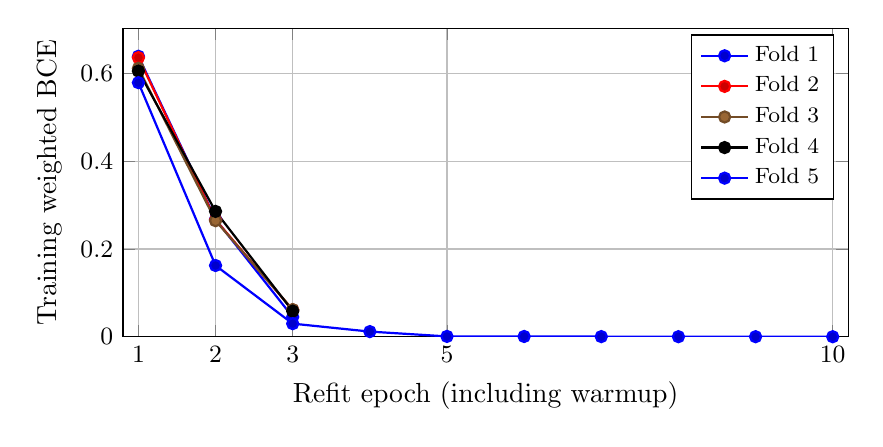
\begin{tikzpicture}
\begin{axis}[width=.89\linewidth,height=5.5cm,xmin=.8,xmax=10.2,ymin=0,
 xlabel={Refit epoch (including warmup)},ylabel={Training weighted BCE},grid=major,
 xtick={1,2,3,5,10},legend style={at={(.98,.98)},anchor=north east,font=\footnotesize},
 tick label style={font=\small}]
\addplot+[mark=*,thick] coordinates {(1.0000000,0.6394369) (2.0000000,0.2678801) (3.0000000,0.0451581)};\addlegendentry{Fold 1}
\addplot+[mark=*,thick] coordinates {(1.0000000,0.6362881) (2.0000000,0.2665114) (3.0000000,0.0613643)};\addlegendentry{Fold 2}
\addplot+[mark=*,thick] coordinates {(1.0000000,0.6120350) (2.0000000,0.2645786) (3.0000000,0.0619980)};\addlegendentry{Fold 3}
\addplot+[mark=*,thick] coordinates {(1.0000000,0.6056941) (2.0000000,0.2858135) (3.0000000,0.0584639)};\addlegendentry{Fold 4}
\addplot+[mark=*,thick] coordinates {(1.0000000,0.5792978) (2.0000000,0.1624607) (3.0000000,0.0299120) (4.0000000,0.0117932) (5.0000000,0.0007995) (6.0000000,0.0006653) (7.0000000,0.0003786) (8.0000000,0.0001830) (9.0000000,0.0001541) (10.0000000,0.0001204)};\addlegendentry{Fold 5}
\end{axis}\end{tikzpicture}
\caption{Last-block 외부 학습 집합 전체의 재적합 손실. 첫 epoch는 head-only warmup이다.
이는 epoch 중 가중 BCE의 누적 평균이며 epoch 종료 후 고정 모델의 평가 손실이 아니다.}
\end{figure}
이력은 주어진 학습 집합에 적합되는 양상을 보여줄 뿐 외부 일반화의 증거는 아니다.
작은 훈련 손실로 임계값을 바꾸거나 외부 평가 성능을 대체하지 않는다.
내부 모든 후보의 전체 trajectory와 validation loss는 저장되지 않았으므로
이 그림만으로 모든 후보의 과적합 시점을 판정할 수 없다.

\subsection{전체 코호트 최종 모델}
외부 평가 뒤 전체 304명에 별도 3-fold 내부 선택을 실시하여
인코더 LR $10^{-5}$, weight decay $0.01$, 총 3 epoch를 선택하였다.
Head-only는 인코더 LR 0, 같은 decay, 총 5 epoch를 선택하였다.
선택 평균 내부 BA는 last-block 79.68\%, head-only 79.19\%지만 후보 선택에 사용한 점수이므로
새로운 독립 평가 성능으로 보고하지 않는다.
두 최종 모델은 각각 전체 코호트로 다시 적합되었고 새로운 독립 시험 집합이 없다.
각 최종 파일은 약 9.27 MiB이며, 인코더/head, 정규화 buffer, 입력 규약,
초기 체크포인트 식별자와 학습 참가자 목록을 포함한다.
optimizer 상태가 없어 중단 시점의 optimizer를 그대로 이어가는 resume 파일은 아니다.

\subsection{한계와 필요한 후속 검증}
\begin{enumerate}
 \item \textbf{28명 ET와 단일 코호트.} 가중치와 층화는 정보 부족을 제거하지 않는다.
 외부 기관/장치/프로토콜에서의 검증과 ET 표본 확대가 필요하다.
 \item \textbf{모드별 선택과 제한된 탐색.} Head-only 대조군은 완료했지만
 각 모드에서 epoch를 따로 선택했다. 고정 epoch의 적응 효과나 다른 seed/탐색 범위로
 일반화하지 않는다. 한 번의 동일 seed 재실행은 이러한 불확실성을 해소하지 않는다.
 \item \textbf{임계값과 비용.} 이번 결과는 고정 점수 0에서의 비교다.
 다른 운영점을 검토하려면 목표 민감도/특이도와 오분류 비용을 먼저 정하고
 내부 자료에서만 임계값을 선택한 뒤 새 외부 평가를 해야 한다.
 \item \textbf{불균형 지표의 역할.} PR-AUC/AP는 ET 검출 precision을 반영하지만
 양성 비율에 의존한다. BA, MCC, G-mean과 클래스별 분모를 함께 제시해야 한다.
 \item \textbf{확률 및 해석.} logit은 보정된 확률이 아니며,
 이번 모델에서 시간적 주파수 안정성이나 과제 상호작용의 임상적 기전을 직접 추론할 수 없다.
\end{enumerate}
\clearpage

\appendix
\section{외부 분할과 재현 설정}\label{app:splits}
\begin{table}[H]\centering\small
\caption{저장된 참가자 분할과 모델 seed. 모든 방법의 분할은 정확히 같다.}
\begin{tabular}{@{}rrrrrr@{}}\toprule
Fold & 학습 PD & 학습 ET & 평가 PD & 평가 ET & 모델 seed\\\midrule
1 & 220 & 23 & 56 & 5 & 2347327255 \\
2 & 221 & 22 & 55 & 6 & 952542970 \\
3 & 221 & 22 & 55 & 6 & 360942606 \\
4 & 221 & 22 & 55 & 6 & 1634018698 \\
5 & 221 & 23 & 55 & 5 & 3142294584 \\
\bottomrule\end{tabular}
\end{table}
\begin{table}[H]\centering\small
\caption{실행 manifest에 기록된 소프트웨어 버전.}
\begin{tabular}{@{}ll@{}}\toprule
소프트웨어 & 버전\\\midrule
Python & 3.12.13\\
NumPy / SciPy & 2.3.5 / 1.17.1\\
scikit-learn & 1.9.1\\
PyTorch & 2.14.1\\
mantis-tsfm / safetensors & 1.1.0 / 0.8.0\\
threadpoolctl & 3.7.0\\\bottomrule
\end{tabular}
\end{table}
실행 명령은 프로젝트 루트 기준으로 다음과 같다.
이 명령은 완료 실행의 재현 정보를 기록한 것이며 보고서 작성 중 실행하지 않았다.
\begin{lstlisting}
.venv-transformer/bin/python -m sota_pd_et.evaluate_mantis_finetune \
  --input-set all --mode last-block --device auto \
  --compare-to artifacts/pads_mantis_v2 \
  --fit-final --save-outer-models

.venv-transformer/bin/python -m sota_pd_et.evaluate_mantis_finetune \
  --input-set all --mode head-only --encoder-lrs 0 --device auto \
  --compare-to artifacts/pads_mantis_v2 \
  --fit-final --save-outer-models
\end{lstlisting}
진행 막대는 초기 채널 특징 추출, 모드별 24/42회 적합, epoch, 참가자, 검증/외부 평가를 표시한다.
진행 표시 자체는 수치 학습 규칙을 바꾸지 않는다.
이 실행은 각 외부 평가 완료 뒤 \code{test_predictions.csv}, \code{metrics.json},
내부 선택/탐색 결과, 재적합 이력과 \code{model.pt}를 저장했다.
각 실행에서 5개 외부 모델과 전체 코호트 최종 모델이 모두 존재함을 확인했다.
실행기는 자동 resume를 지원하지 않으며, 저장 모델에 optimizer 상태도 없다.

\textbf{초기 체크포인트 SHA-256.}
\begin{quote}\footnotesize
\code{config.json}:\\
\path{f28885b7aa662cedcaf5627659fc0fba9cf8ee49d5b991280522e04fa5b1ae80}\\[.4em]
\code{model.safetensors}:\\
\path{49d46d9a49cccdc87c46f4e0088fa52c0a6ef7eb4c13de5cc9815426b7b17ab1}
\end{quote}
\clearpage

\section{내부 탐색 전체 요약}
아래 값은 후보 선택 자료이며 외부 일반화 성능이 아니다.
각 행의 weight decay는 0.01이다. Final은 전체 코호트의 별도 내부 선택이다.
각 LR trajectory는 최대 10 epoch까지 학습하고 3/5/10 epoch에서 평가하므로 독립 반복이 아니다.
\begingroup\footnotesize\renewcommand{\arraystretch}{.95}
\begin{longtable}{@{}llrrrrr@{}}
\caption{내부 후보 54개(Head-only 18개, Last-block 36개). SD는 내부 fold 간 기술적 변동이다.}\\
\toprule 모드 & Fold & 인코더 LR & Epoch & 평균 BA(\%) & BA SD(pp) & Pooled AUROC\\\midrule\endfirsthead
\toprule 모드 & Fold & 인코더 LR & Epoch & 평균 BA(\%) & BA SD(pp) & Pooled AUROC\\\midrule\endhead
\bottomrule\endfoot
Head & 1 & 0e+00 & 3 & 81.52 & 7.98 & 0.8937 \\
Head & 1 & 0e+00 & 5 & 79.16 & 1.52 & 0.8953 \\
Head & 1 & 0e+00 & 10 & 77.01 & 5.64 & 0.8939 \\
Head & 2 & 0e+00 & 3 & 83.34 & 2.25 & 0.9441 \\
Head & 2 & 0e+00 & 5 & 81.54 & 1.23 & 0.9377 \\
Head & 2 & 0e+00 & 10 & 85.50 & 5.95 & 0.9383 \\
Head & 3 & 0e+00 & 3 & 78.03 & 9.53 & 0.8809 \\
Head & 3 & 0e+00 & 5 & 78.93 & 9.18 & 0.8824 \\
Head & 3 & 0e+00 & 10 & 81.99 & 6.48 & 0.8832 \\
Head & 4 & 0e+00 & 3 & 80.18 & 4.63 & 0.9111 \\
Head & 4 & 0e+00 & 5 & 78.72 & 3.60 & 0.8869 \\
Head & 4 & 0e+00 & 10 & 82.91 & 2.57 & 0.8906 \\
Head & 5 & 0e+00 & 3 & 83.65 & 6.12 & 0.9237 \\
Head & 5 & 0e+00 & 5 & 83.18 & 8.65 & 0.9359 \\
Head & 5 & 0e+00 & 10 & 81.34 & 4.33 & 0.9333 \\
Head & Final & 0e+00 & 3 & 77.01 & 8.76 & 0.9071 \\
Head & Final & 0e+00 & 5 & 79.19 & 4.29 & 0.9053 \\
Head & Final & 0e+00 & 10 & 78.10 & 4.17 & 0.9073 \\
Last & 1 & 1e-05 & 3 & 76.35 & 16.98 & 0.8951 \\
Last & 1 & 1e-05 & 5 & 65.60 & 13.07 & 0.8781 \\
Last & 1 & 1e-05 & 10 & 63.06 & 14.61 & 0.8974 \\
Last & 1 & 3e-05 & 3 & 73.93 & 15.27 & 0.8828 \\
Last & 1 & 3e-05 & 5 & 67.22 & 16.42 & 0.8891 \\
Last & 1 & 3e-05 & 10 & 65.37 & 18.66 & 0.8889 \\
Last & 2 & 1e-05 & 3 & 79.35 & 3.18 & 0.9459 \\
Last & 2 & 1e-05 & 5 & 68.66 & 10.57 & 0.9369 \\
Last & 2 & 1e-05 & 10 & 71.42 & 13.05 & 0.9513 \\
Last & 2 & 3e-05 & 3 & 67.48 & 10.43 & 0.9364 \\
Last & 2 & 3e-05 & 5 & 71.42 & 13.05 & 0.9418 \\
Last & 2 & 3e-05 & 10 & 69.33 & 5.39 & 0.9461 \\
Last & 3 & 1e-05 & 3 & 74.64 & 8.35 & 0.8937 \\
Last & 3 & 1e-05 & 5 & 73.58 & 6.65 & 0.9087 \\
Last & 3 & 1e-05 & 10 & 73.35 & 6.87 & 0.9155 \\
Last & 3 & 3e-05 & 3 & 74.25 & 6.06 & 0.9033 \\
Last & 3 & 3e-05 & 5 & 73.35 & 6.33 & 0.9074 \\
Last & 3 & 3e-05 & 10 & 74.25 & 6.06 & 0.9109 \\
Last & 4 & 1e-05 & 3 & 69.31 & 14.58 & 0.9085 \\
Last & 4 & 1e-05 & 5 & 66.27 & 9.32 & 0.8896 \\
Last & 4 & 1e-05 & 10 & 66.20 & 12.37 & 0.8945 \\
Last & 4 & 3e-05 & 3 & 64.12 & 9.19 & 0.8904 \\
Last & 4 & 3e-05 & 5 & 66.88 & 11.72 & 0.8949 \\
Last & 4 & 3e-05 & 10 & 64.34 & 8.67 & 0.9027 \\
Last & 5 & 1e-05 & 3 & 77.13 & 8.71 & 0.9254 \\
Last & 5 & 1e-05 & 5 & 77.22 & 8.15 & 0.9528 \\
Last & 5 & 1e-05 & 10 & 74.76 & 4.93 & 0.9542 \\
Last & 5 & 3e-05 & 3 & 75.59 & 7.98 & 0.9361 \\
Last & 5 & 3e-05 & 5 & 75.36 & 11.94 & 0.9490 \\
Last & 5 & 3e-05 & 10 & 81.31 & 4.95 & 0.9548 \\
Last & Final & 1e-05 & 3 & 79.68 & 3.58 & 0.9064 \\
Last & Final & 1e-05 & 5 & 73.74 & 9.78 & 0.9077 \\
Last & Final & 1e-05 & 10 & 70.40 & 9.97 & 0.9092 \\
Last & Final & 3e-05 & 3 & 72.44 & 11.87 & 0.9191 \\
Last & Final & 3e-05 & 5 & 72.25 & 7.23 & 0.9139 \\
Last & Final & 3e-05 & 10 & 72.25 & 7.23 & 0.9151 \\
\end{longtable}
\endgroup
\clearpage

\section{저장 자료 감사와 보고서 재생성}
보고서 생성기는 학습 함수, 모델 생성 함수나 순전파를 호출하지 않는다.
독립적으로 다시 확인한 항목은 다음과 같다.
\begin{enumerate}
 \item 304명의 고유 ID/정답, ET 28명, PD 설명의 ET 언급 8명과 공식 라벨 유지.
 \item 외부 5개 평가 집합의 완전 분할, 내부 3개 집합의 분리와 ID/인덱스 일치.
 네 방법의 참가자 순서, 데이터 출처, 전체 중첩 분할의 정확한 일치.
 \item 방법별 참가자 304명당 외부 점수 한 개, 유한 점수, 엄격한 $s>0$ 판정,
 개별 fold 파일과 통합 OOF 파일의 일치.
 \item 모든 저장 평가 지표, 혼동행렬과 평균 fold 지표의 재계산.
 원본 저장값은 절대 오차 $10^{-12}$ 이내로 일치했다.
 PR-AUC와 G-mean은 저장 점수에서 추가 계산했으며 PR-AUC/AP의 적분 합도 검증했다.
 \item 모드별 내부 후보(3/6개)의 grid, 최대 평균 BA와 동률 규칙, 선택 후보의 내부 OOF 지표,
 선택 epoch만큼의 재적합 이력과 모드별 warmup 동작.
 선택되지 않은 후보의 개별 참가자 점수는 저장되지 않아 후보 요약을 완전히 재구성할 수 없다.
 \item 611개 데이터 파일의 SHA-256, 초기 체크포인트 및 고정 특징 cache의 해시/형상,
 실행별로 보관한 소스 28개 파일의 해시와 ZIP CRC.
 세 실행의 소스 snapshot과 현재 평가 코드 28개가 모두 일치했다.
 \item 세 실행의 18개 모델 파일을 \code{torch.load(weights_only=True)}로 읽어
 학습 ID, 선택 설정, 초기 가중치 식별자, 세 블록 구조와 유한 텐서를 확인했다.
 각 실행의 외부 모델 5개와 최종 모델의 평균/표준편차 buffer가
 해당 학습 참가자의 초기 고정 특징 통계와 정확히 일치했다.
 모든 비학습 인코더 텐서가 초기 가중치와 같고, last-block의 세 번째 블록이
 실제로 변경되었음을 확인했다. 이전/새 last-block의 저장 state tensor도 모두 같았다.
 모델 예측을 재실행하여 저장 점수를 재현하는 검사는 하지 않았다.
\end{enumerate}

주 실행 두 개의 상대 경로는 다음과 같다. 이전 last-block의 경로와 식별자는
표~\ref{tab:runs} 및 감사 JSON에 기록한다.
\begin{quote}\small
\path{artifacts/pads_mantis_v2_finetuned/20261109T032315873662Z/}\\
\path{artifacts/pads_mantis_v2_finetuned/20261109T041659480074Z/}
\end{quote}
보고서 폴더의 \code{verification.json}은 세 실행 manifest, 재계산 지표,
대응 결과, bootstrap 규약, 재실행 동일성 확인 및 핵심 파일 해시를 포함한다.
\code{metrics.csv}는 PR-AUC/AP를 구분한 방법별 지표를 제공한다.
\code{fold_metrics.csv}는 네 방법의 20개 외부 fold 결과를 제공한다.
\code{report.tex}는 표와 그래프 좌표 및 참고문헌을 내장한 독립 문서다.
데이터나 모델 파일 없이 XeLaTeX로 컴파일할 수 있다.
\begin{lstlisting}
cd MantisV2_FineTune_Report
latexmk -xelatex -interaction=nonstopmode -halt-on-error \
  -outdir=../tmp/pdfs/mantis_finetune report.tex
\end{lstlisting}
원 실행과 비교군 자료가 같은 프로젝트 구조에 있으면 다음 명령으로 감사와 원고를 재생성한다.
이 작업은 저장 자료 분석이며 재학습이 아니다.
\begin{lstlisting}
.venv-transformer/bin/python MantisV2_FineTune_Report/build_report.py
\end{lstlisting}
\clearpage

\begin{thebibliography}{9}\small
\bibitem{pads} J. Varghese, A. Brenner, L. Plagwitz, C. van Alen, M. Fujarski,
 T. Warnecke. PADS -- Parkinsons Disease Smartwatch dataset, version 1.0.0.
 PhysioNet, 2024. \url{https://doi.org/10.13026/m0w9-zx22}.
\bibitem{padsstudy} J. Varghese et al. Machine Learning in the Parkinson's disease smartwatch
 (PADS) dataset. \emph{npj Parkinson's Disease} 10, 9, 2024.
 \url{https://doi.org/10.1038/s41531-023-00625-7}.
\bibitem{mantis} V. Feofanov, S. Wen, J. Zhang, L. Pan, I. Redko.
 MantisV2: Closing the Zero-Shot Gap in Time Series Classification with Synthetic Data
 and Test-Time Strategies. arXiv:2602.17868, 2026.
 \url{https://arxiv.org/abs/2602.17868}.
\bibitem{adamw} I. Loshchilov, F. Hutter. Decoupled Weight Decay Regularization.
 ICLR, 2019. \url{https://arxiv.org/abs/1711.05101}.
\bibitem{multirocket} C. W. Tan, A. Dempster, C. Bergmeir, G. I. Webb.
 MultiRocket: Multiple pooling operators and transformations for fast and effective
 time series classification. \emph{Data Mining and Knowledge Discovery}, 2022.
 \url{https://doi.org/10.1007/s10618-022-00844-1}.
\bibitem{hydra} A. Dempster, D. F. Schmidt, G. I. Webb.
 HYDRA: Competing convolutional kernels for fast and accurate time series classification.
 \emph{Data Mining and Knowledge Discovery}, 2023.
 \url{https://doi.org/10.1007/s10618-023-00939-3}.
\bibitem{mcc} D. Chicco, G. Jurman. The advantages of the Matthews correlation coefficient
 (MCC) over F1 score and accuracy in binary classification evaluation.
 \emph{BMC Genomics} 21, 6, 2020. \url{https://doi.org/10.1186/s12864-019-6413-7}.
\bibitem{sklearnap} scikit-learn developers. \code{average_precision_score} and
 \code{precision_recall_curve}, version 1.9.1 documentation. Accessed 2026-11-09.
 \url{https://scikit-learn.org/stable/modules/generated/sklearn.metrics.average_precision_score.html};
 \url{https://scikit-learn.org/stable/modules/generated/sklearn.metrics.precision_recall_curve.html}.
\end{thebibliography}
\end{document}
